% \begin{savequote}[8cm]
% \textlatin{Neque porro quisquam est qui dolorem ipsum quia dolor sit amet, consectetur, adipisci velit...}

% There is no one who loves pain itself, who seeks after it and wants to have it, simply because it is pain...
%   \qauthor{--- Cicero's \textit{de Finibus Bonorum et Malorum}}
% \end{savequote}

\chapter{\label{ch:4-dents}Monte Carlo Tree Search With Boltzmann Exploration} 

    \minitoc

    This chapter considers MCTS algorithms for planning in single-objective environments, where the algorithm may consider a secondary entropy objective for exploration. In the maximum entropy setting the optimal soft policy takes the form of a Boltzmann distribution (Section \ref{sec:2-3-1-merl}), and the chapter will predominantly discuss MCTS algorithms whose search policies take the form of Boltzmann distributions. Question \entropyq, about how entropy can be used soundly in MCTS planning algorithms is answered here, and the foundations are laid for answering \contextq\ewe in Chapter \ref{ch:6-simplexmaps}.
    
    The discussion will focus on the exploration setting for reinforcement learning (see Section \ref{sec:2-3-rl} and Figure \ref{fig:4:rl_overview}), where agents are assessed purely on the recommendations it makes, rather than what actions it explored in simulation.
    
    \begin{figure}
        \centering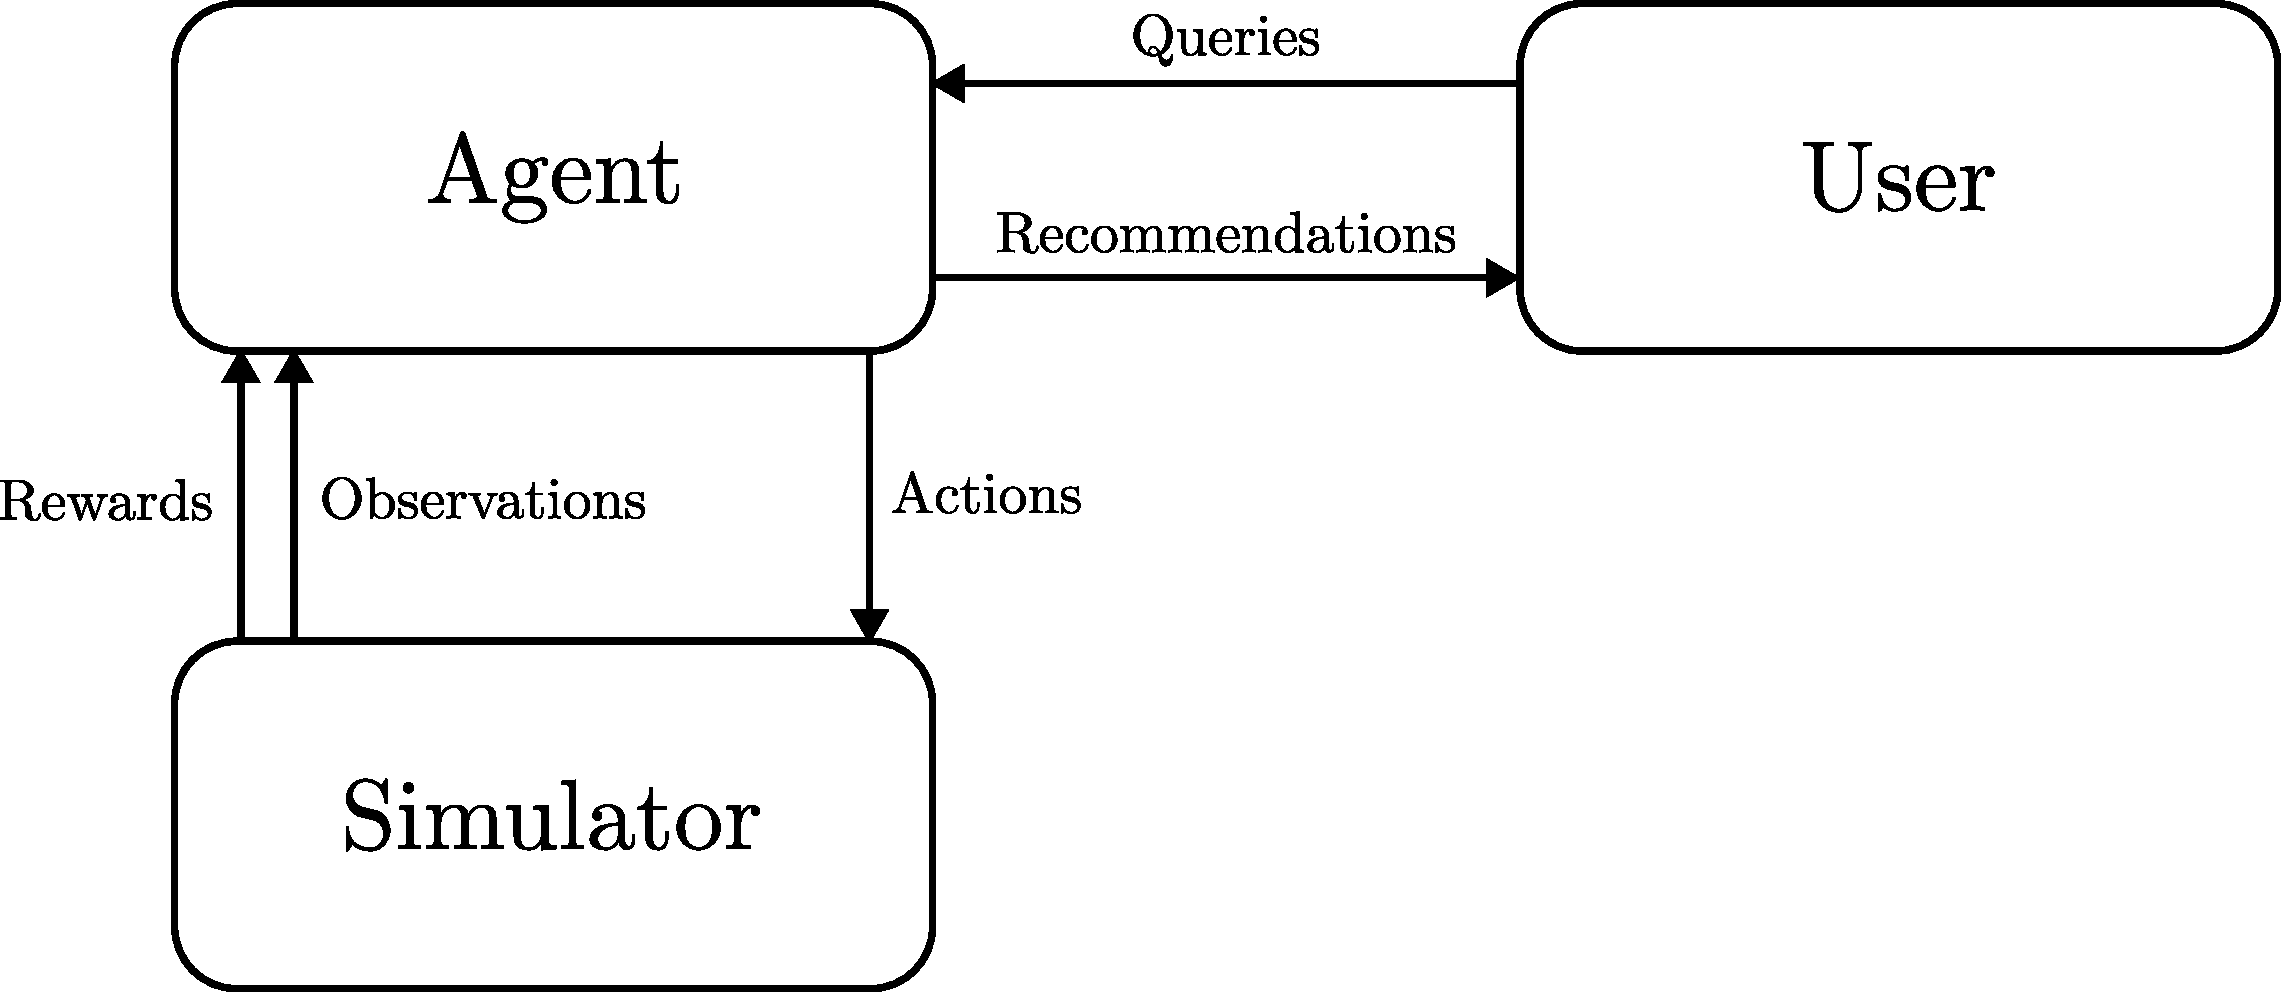
\includegraphics[width=0.75\textwidth]{figures/ch4/rl_overview.pdf} 
        \caption[Exploration setting in reinforcement learning.]{Exploration setting in reinforcement learning (edited from Figure \ref{fig:2:rl_overview}), where the agent is only assessed on the recommendations that it provides, and is not penalised for considering poor actions in the simulator. So this setting places greater emphasis on exploration over exploitation.}
        \label{fig:4:rl_overview}
    \end{figure}
    
    Entropy is widely used in the reinforcement learning literature, commonly introduced to promote exploration and discourage convergence to suboptimal deterministic policies \cite{ppo,deep_energy_policies,a3c,reinforce_ment}. MENTS (Section \ref{sec:2-4-3-ments}), RENTS and TENTS (Section \ref{sec:3-3-3-rents-some-tents}) are all MCTS algoritms that optimise for maximum entropy objectives. While RENTS and TENTS will be considered as baselines in empirical experiments, MENTS will be used to facilitate and provide discussion around the use of entropy and maximum entropy objective.

    Section \ref{sec:4-1-intro} discusses limitations of existing MCTS algorithms in the exploration setting, motivating the work covered in the remainder of the chapter. Additionally, the planning framework is formally defined so that the algorithms can be theoretically analysed using \textit{simple regret}.
    
    In Section \ref{sec:4-2-boltzmannsearch} the \textit{Boltzmann Tree Search} (BTS) and \textit{Decaying ENtropy Tree Search} (DENTS) algorithms are defined. Section \ref{sec:4-2-3-stoch_search_policies} additionally discusses some useful properties of using a stochastic search policy in MCTS, such as naturally including prior knowledge through mixed policies, and how the Alias method (Section \ref{sec:2-6-sampling}) can be used to improve on computational complexity to answer \complexityq.

    Section \ref{sec:4-3-toyenvs} considers some theoretical MDPs, which are used to empirically demonstrate the limitations of the existing MCTS algorithms, and are additionally used to provide discussion around \entropyq.

    Results on grid world environments and the game of Go are given in section \ref{sec:4-4-results}. 

    Finally, in Section \ref{sec:4-5-theory} the main theoretical analysis and proofs are given. Convergence properties of MENTS, BTS and DENTS are proven to answer \entropyq.

    \htodo{After finished writing, do another pass through neurips paper and check no results/writing missing from thesis that really should be included. (Thinking about some of the frozen lake plots in the appendix when writing this.)}
    







\section{Introduction and Motivation}
\label{sec:4-1-intro}

\newcommand{\secfouronestate}{s^{(2,2)}}.

    In this section a grid world shortest path problem will be used to discuss the behaviour of UCT and MENTS in the exploration setting, and highlight some limitations of these algorithms. In this grid world the agent may move deterministically in any cardinal direction, North/East/South/West, provided it stays on the grid. The agent starts at the origin $(0,0)$ and the goal is to reach the other side of the grid, at $(G-1,G-1)$, where $G$ is the grid size. The cost of a path is equal to its length, and an optimal policy will always select actions that move the agent \texttt{UP} or \texttt{RIGHT}. 

    This MDPs can be defined formally:
    \begin{align}
        \cl{S} &= \{(x,y)\in\bb{N}^2 | x,y \in [0,G]\} \\
        s_0 &= (0,0) \\
        \cl{A} &= \{(1,0),(0,-1),(-1,0),(0,1)\} = \{\texttt{UP},\texttt{LEFT},\texttt{DOWN},\texttt{RIGHT}\} \\
        \text{clip}((x,y)) &= \left(\max(\min(x,G-1),0), \max(\min(y,G-1),0)\right) \\
        p(s'|s,a) &= \begin{cases}
            \one[s'=s] & \text{if } s=(G-1,G-1) \\
            \one[s'=\text{clip}(s+a)] & \text{otherwise}
        \end{cases} \\
        H &= 6G \\
        R(s,a) &= -1 
    \end{align}

    In Section \ref{sec:4-4-results} similar grid world problems will be considered with greater complexities, such as sparse rewards and stochastic transition distributions.

    
    
    \begin{figure}
        \centering
        \begin{subfigure}[b]{0.49\textwidth}
            \centering
            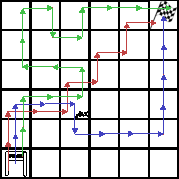
\includegraphics[width=\textwidth]{figures/ch4/grid_world_sec_1.pdf}
            \caption{Some possible paths from start to finish.\\ \ewe}
            \label{fig:4:shortest_path_intro_a}
        \end{subfigure}
        \hfill
        \begin{subfigure}[b]{0.49\textwidth}
            \centering
            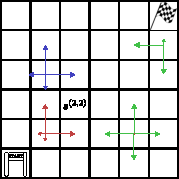
\includegraphics[width=\textwidth]{figures/ch4/grid_world_sec_1_entropy.pdf}
            \caption{Optimal policy with the maximum entropy objective for varying temperatures.}
            \label{fig:4:shortest_path_intro_b}
        \end{subfigure}
        \caption[An example grid world shortest path problem.]{An example grid world shortest path problem. (a) shows three possible paths, that could be explored by UCT. The red path shows one possible optimal path from the start to finish (cost of 10). The blue path shows a near optimal path (cost of 12), and the green path shows a suboptimal path (cost of 16). Supposing UCT has searched the blue and green paths, when the UCT search policy selects actions at state $\secfouronestate$, it will often pick action \texttt{DOWN} over action \texttt{UP}, as the Q-value estimates it has are $\Quct(\secfouronestate,\texttt{DOWN})=-8$ and $\Quct(\secfouronestate,\texttt{UP})=-12$. (b) shows the probability of sampling actions from the optimal soft policy for varying temperature $\alpha$. Red corresponds to a small value of $\alpha$, and is close to the optimal standard policy. Blue corresponds to a mid-range value of $\alpha$ where the optimal policy will still try to reach the goal, but still act randomly to obtain entropy reward. Green corresponds to a large value of $\alpha$, where obtaining entropy reward outweighs ever reaching the goal, and the optimal soft policy is nearly uniform. For large values of entropy the optimal soft policy actively avoids reaching the goal that will end the trial, and will have a slight preference to stay near the middle of the grid, as there are fewer available actions at the edges and corners (less entropy available). \todo{clean up alignment of arrows in figs and make state label clearer in fig a}}
        \label{fig:4:shortest_path_intro}
    \end{figure}
    
    \begin{figure}
        \centering
        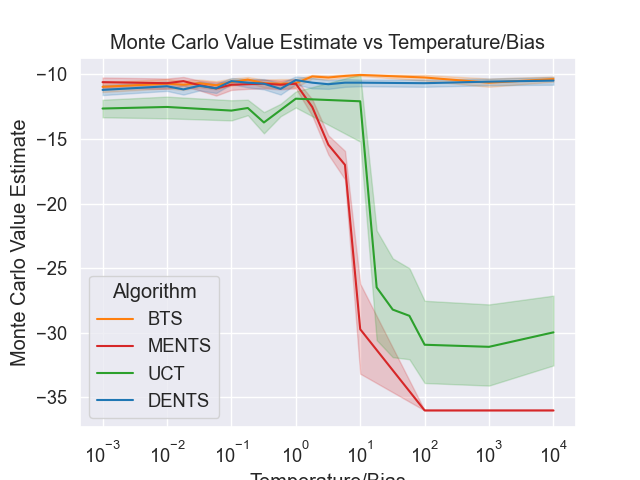
\includegraphics[width=0.6\textwidth]{figures/ch4/grid_world_sec_1_results.png}
        \caption[Results on the example grid world problem for a variety of bias and temperature parameters.]{Results on the example grid world problem for a variety of UCT bias and temperature parameters. For comparison, the Boltzmann Tree Search (BTS) and Decaying ENtropy Tree Search (DENTS) algorithms defined in Section \ref{sec:4-2-boltzmannsearch} are also shown. Each algorithm was run for 5000 trials, and results were averaged over 25 repeated experiments. UCT is able to find the optimal solution in some of the repeats with a bias of 10, but for larger biases 5000 trials was not enough to converge. MENTS successfully finds the shortest path of length 10 for small values of $\alphaments$, but for values in the inteval $[1,100)$ the entropy objective encourages a scenic route to the goal, and for values $100+$ acting randomly to gain entropy reward far outweighs reaching the goal. \todo{Make sure can actually see x-axis label (Temperature/Bias)}}
        \label{fig:4:shortest_path_intro_results}
    \end{figure}


    \subsection{UCT}

        The UCT algorithm (Section \ref{sec:2-4-2-uct}) is designed in the traditional reinforcement learning setting described in Section \ref{sec:2-3-rl}, where the UCT agent aims to minimise the cumulative regret. Thus UCT makes a trade off between exploration and exploitation during it trials, and as such will frequently choose the same action to exploit, which can result in it getting stuck in local optima when rewards are sparse or not informative. 

        A sparse reward is where the reward signal is infrequent, that is, most actions give a reward of zero. In the shortest path example, the reward is dense but relatively uninformative, as the immediate cost of taking any action is the same. 

        In Figure \ref{fig:4:shortest_path_intro_a} the shortest path problem is depicted, with an optimal path shown in red, and two paths that UCT may have explored in blue and green. When UCT is selecting an action to take from state $\secfouronestate$, it will consider the value estimates $\Quct(\secfouronestate,\texttt{DOWN})\approx -8$ and $ \Quct(\secfouronestate,\texttt{UP})\approx -12$ (note that at state $\secfouronestate$ the agent has already taken 4 steps along the path). As the Q-value estimate for taking the suboptimal action \texttt{DOWN} is higher, UCT will most frequently select this action from state $\secfouronestate$. 

        UCT will select every action infinitely often (that is, $N(s,a)\rightarrow \infty$ for all reachable $s,a$) and in theory will eventually converge to the optimal policy. However, in practise this could take a long time. In Section \ref{sec:4-3-toyenvs} a theoretical MDP is considered where UCT needs much more than $\exp(|\cl{S}|)$ trials for the search policy to converge to the optimal policy.

        In Figure \ref{fig:4:shortest_path_intro_results} the performance of UCT after 5000 trials is given for a range of values of the UCT bias parameter $\buct$. This bias parameter controls the amount of exploration that UCT performs, and as the bias parameter is increased UCT will explore more. It can be seen that for low values of the bias parameter UCT is stuck in a suboptimal solution. When the bias parameter is increased UCT sufficiently explores to find the optimal policy. Finally, as UCT uses sample averages, for a very large bias parameter, 5000 trials is not sufficient enough for the average return value estimates to converge. Note that the (Q-)values of UCT can also be written as:
        \begin{align}
            \Vuct(s) &= \sum_{a \in \cl{A}} \frac{N(s,a)}{N(s)}\Quct(s,a), \\
            \Quct(s,a) &= R(s,a) \sum_{s' \in \suc{s}{a}} \frac{N(s')}{N(s,a)}\Vuct(s,a),
        \end{align} 
        and so the empirical distribution $\frac{N(s,a)}{N(s)}$ needs to a converge to a one hot distribuion before the value estimates can converge to the optimal values.
        
        \hide{\todo{This later issue can be resolved by using MaxUCT instead. Add? Also add in results Section 4.4?}}


    
    
    \subsection{MENTS}

        One can argue that when using the maximum entropy objective, it is possible to recover the standard objective by setting the temperature parameter to zero, or an infitesimally small value. However, in practise, setting $\alpha$ to a tiny value will nullify the exploration advantages of using entropy. Considering the other extreme, when a very large temperature is used, entropy becomes the dominant objective in the maximum entropy objective, and the optimal soft policy will be (almost) uniform. 

        The optimal soft policy for a large temperature may be very different to the optimal policy for the standard objective. In cases such as this, it can be said that the maximum entropy objective is \textit{misaligned} with the standard objective. More precisely, the maximum entropy objective is misaligned when the policy $\pi^*_{\sft,\text{eval}}(s) = \argmax_{a'} \pi^*_{\sft}(a'|s)$ that would be followed at test time differs from the optimal standard policy $\pi^*(s)$.
        
        For a more concrete example of this phenominon, consider the shortest path example and what the optimal soft policy look like at a state next to the goal? The agent can either reach the goal in the next step, or, alternatively move away from the goal so that it can collect more entropy reward. This is depicted in Figure \ref{fig:4:shortest_path_intro_b} in purple.   

        Hence, when using the maximum entropy objective the temperature parameter often needs to be carefully tuned to the MDP. Using too small of a value will nullify the exploration benefits, and using too large of a value will result in the maximum entropy objective being misaligned with the standard objective. In Section \ref{sec:4-3-toyenvs} a theoretical MDP is considered where the temperature parameter needs to be made prohibitively small to avoid the maximum entropy objective from being misaligned. 

        In Figure \ref{fig:4:shortest_path_intro_results} the performance of MENTS after 5000 trials is given for a range of values of the temperature parameter $\alphaments$. For temperature values up to a value of 1, a close to optimal path is found in the shortest path problem. In the range of temperatures between 1 and 100, it becomes more beneficial for MENTS to act randomly to obtain entropy but will still tend to move towards the goal, and beyond a value of 100 it becomes much more valueable to act randomly and optimise for entropy. 

        Building off this intuition, a good rule of thumb when using the maximum entropy objective is to set the temperature parameter large enough to gain an exploration benefit, but small enough to avoid misalignment issues. Additionally, the threshold for which the maximum entropy objective will become misaligned is dependent on the MDP itself, considering that a uniform policy over $|\cl{A}|$ actions has an entropy of $\log(|\cl{A})$. Generally this means that the temperature will need to be carefully tuned for any new MDP that it is used with.
        
        Furhermore, in Section \ref{sec:4-3-toyenvs}, a theoretical MDP will be constructed where MENTS will either suffer from the issue of the entropy objective misalignment, or the temperature must be set to a small value that does not effectively utilise the entropy exploration. 
        
        While only the MENTS algorithm has been discussed in this section, the issue arises from mixing entropy into the scalar objective. Similar issues still arise no matter the form of entropy considered.



    \subsection{Simple Regret and Consistency}

        \todo{Move to chapter 2 in RL section and add cumulative regret. Call subsection regret and consistency.}

        Now \textit{simple regret} is defined, which will be used motivate and analyse the algorithms developed. The simple regret of a policy is the difference between the value of the policy and optimal value of the policy (Equation (\ref{eq:4:simple_regret})). By definition, the optimal policy achieves a simple regret of zero, and an MCTS algorithm is considered \textit{consistent} if it's expected simple regret tends to zero. In plain english, an algorithm is consistent if left to run forever it would eventually output an optimal policy. An implication of consistency is that if an algorithm can be run for longer, then it is expected to improve on its solution.

        While \textit{cumulative regret} has been used to motivate and analyse algorithms such as UCT, it is not the most appropriate measure for the exploration setting. In the exploration setting, the agent is only assessed on the recommendations it makes, and is not penalised for considering poor actions in the simulator. See Figure \ref{fig:4:planning_problem} for the formal setup of the exploring planning problem for MDPs. As such, the focus of this chapter will be on the (expected) simple regret of the algorithms developed.

        % \todo{Talk about the setup we're using. Probably want to try motive similarly to DENTS paper, and recall the diagram from} \ref{sec:2-3-rl}. \todo{Say that in fig below that normally step 3 is not considered} \todo{Neurips paper says: ``In this work, we consider scenarios where MCTS methods are used with a simulator to plan how an
        % agent should act'' in intro, and ``UCB [1] is frequently used in MCTS methods to minimise cumulative regret during the tree search.
        % Cumulative regret is most appropriate in scenarios where the actions taken during tree search have an
        % associated real-world cost. However, MCTS methods often use a simulator during the tree search,
        % where the only significant real-world cost is associated with taking the recommended action after the
        % tree search. In such scenarios, simple regret [7, 8] is more appropriate for analysing the performance
        % of algorithms, as it only considers the cost of the actions that are actually executed. Under simple
        % regret, algorithms are not penalised for under-exploiting during the search, thus can explore more,
        % which leads to better recommendations by allowing algorithms to confirm that bad actions are indeed
        % of lower value.'' in the simple regret section} 

        \begin{figure}
            \begin{tcolorbox}
                Parameters: An MDP $\cl{M}$.
                \begin{itemize}
                    \item For each round $m=1,2,...$:
                    \begin{enumerate}
                        \item the agent produces a search policy $\pi^m$ to follow;
                        \item the environment samples a trajectory $\tau\sim\pi^m$ (including rewards $r_t=R(s_t,a_t)$ for each $s_t,a_t$ pair in $\tau$);
                        \item the agent produces a recommendation policy $\psi^m$;
                        \item if the environment sends a stop signal, then the game ends, otherwise the next round starts.
                    \end{enumerate} 
                \end{itemize}
            \end{tcolorbox}
            \caption[The procedure of an exploring planning problem for MDPs]{The procedure of an exploring planning problem for MDPs, where $\psi^m$ is the recommendation policy the agent produces after $m$ trajectories are sampled using the exploration policy $\pi^m$.}
            \label{fig:4:planning_problem}
        \end{figure}

        \begin{defn}
            The \textnormal{simple regret} of a policy $\psi$ at state $s\in\cl{S}$ is the difference between the value of the policy and the optimal value at that state:
            \begin{align}
                \sreg(s,\psi) = V^*(s)-V^{\psi}(s). \label{eq:4:simple_regret}
            \end{align}
        \end{defn}

        Note that the simple regret is a random variable, as it depends on the recommendation policy $\psi$, which itself depends on the random trajectories that are sampled. Hence the expected simple regret will be the main value of interest in the theoretical analysis of Section \ref{sec:4-5-theory}.

        Now that simple regret has been defined, the concept of consistency can be defined formally:

        \begin{defn}
            An agent, that produces recommendation policies $\psi^1,\psi^2,...$ is said to be \textnormal{consistent} if $\bb{E}[\sreg(s,\psi^m)] \rightarrow 0$ as $m\rightarrow \infty$.
        \end{defn}

        Returning to the discussion around UCT and MENTS, now that simple regret and consistency have been defined, it can be shown the UCT is always consistent \todo{cite?}, whereas MENTS is only consistent for a sufficiently small temperature parameter that depends on the MDP (\todo{ref section/theorem, where show MENTS garunteed to converge given a small enough temperature. Maybe quote theorem here?}). Although UCT is consistent, it can take a long time to converge to the optimal policy (as will be seen in \ref{sec:4-3-toyenvs}), and so it is of interest to develop algorithms that can explore more that are also consistent.
    










\section{Boltzmann Search}
\label{sec:4-2-boltzmannsearch}

    This section defines new algorithms, Boltzmann Tree Search (BTS) and Decaying ENtropy Tree Search (DENTS). Following the discussion from Section \ref{sec:4-1-intro}, the design aims of these algorithms are as follows:
    \begin{itemize}
        \item to be as simple to define and implement as UCT and MENTS (i.e. each decision node operates on a multi-armed bandit problem);
        \item be able to explore effectively when rewards are sparse or uninformative;
        \item be able to exploit when necessary (dense informative rewards, large environments or stochastic environments);
        \item can be shown to be consistent for parameters that do not depend on the MDP.
    \end{itemize}

    In Section \ref{sec:4-2-1-bts} BTS is defined, which adapts MENTS to run on the standard objective to arrive at a consistent algorithm. Then Section \ref{sec:4-2-2-dents} defines DENTS which re-introduces entropy as an exploration bonus while maintaining consistency.



    
    \subsection{Boltzmann Tree Search}
    \label{sec:4-2-1-bts}

        The \textit{Boltzmann Tree Search} (BTS) algorithm uses value estimates $\Vbts$ and $\Qbts$ that are computed using \textit{Bellman backups}. Additionally, BTS uses a variable temperature specified by the positive function $\alphabts(x)>0$, and at a decision node $s$ the temperature used will be $\alphabts(N(s))$. BTS promotes exploration through the use of a stochastic Boltzmann search policy.
        
        The search policy of BTS is defined as: 
        %
        \begin{align}
            \pibts(a|s) &= (1-\lambdabts)\rhobts(a|s) + \frac{\lambdabts}{|\cl{A}|}, 
                        \label{eq:4:bts_search_policy} \\ 
            \rhobts(a|s) &\propto \exp\left(\frac{1}{\alphabts(N(s))}\left(\Qbts(s,a)\right)\right).
                        \label{eq:4:bts_value_policy} \\
            \lambda(s,\epsilon) &= \min\left(1, \frac{\epsilon}{\log(e+N(s))}\right) \label{eq:4:lambda}
        \end{align}
        %
        where $\epsbts \in [0,\infty)$ is an exploration parameter. %When $\alphabts(N(s))=0$, equation (\ref{eq:4:bts_value_policy}) is taken to be $\rhobts(a|s)=\one[a=\max_{a'\in\cl{A}} \Qbts(s,a)]$.
        
        Given a trajectory $\tau=(s_0,a_0,r_0,...,s_{h-1},a_{h-1},r_{h-1},s_h)\sim\pibts$ the value estimates are updated for $t=h-1,...,0$:
        \begin{align}
            \Qbts(s_t,a_t) &\leftarrow 
                R(s_t,a_t) + \sum_{s' \in \suc{s_t}{a_t}} \left( \frac{N(s')}{N(s_t,a_t)} \Vbts(s') \right), 
                        \label{eq:4:bts_backup_q} \\ 
            \Vbts(s_t) &\leftarrow \max_{a\in\cl{A}} \Qbts(s_t,a).
                        \label{eq:4:bts_backup_v} 
        \end{align}

        In line with the \thtspp\ewe schema, the values of $\Vbts(s)$ are initialised with the function $\Vinit$ and any missing values of $\Qbts(s,a)$ are completed using the function $\Qinit$. By default these functions can be set to a constant value, or could encorporate prior information, for example with the use of neural networks.
        
        When BTS needs to recommend a policy, it can use it's Q-value estimates:
        %
        \begin{align}
            \psibts(s)=\argmax_{a\in\cl{A}}\Qbts(s,a). \label{eq:4:psibts}
        \end{align}
        %
        Alternatively, the node visit counts can be used in the recommendation policy
        \begin{align}
            \mvbts(s) = \argmax_{a\in\cl{A}} N(s,a). \label{eq:4:mvbts}
        \end{align}

        \newcommand{\norm}{{\text{norm}}}
        Similarly to UCT the best setting of the temperature function will be dependent on the reward scaling. Rather than adding a scaling factor to this parameter, BTS can operate in an \texttt{adaptive\_policy} mode, where the Q-values are normalised to the unit interval before they are used in the policy:
        \begin{align}
            \rhobts(a|s) &\propto \exp\left(\frac{1}{\alphabts(N(s))}\left(\Qbts^{\norm}(s,a)\right)\right). \\
            \Qbts^{\norm}(s,a) &= 
                \frac{\Qbts(s,a)-\min_{a\in\cl{A}}\Qbts(s,a)}{\max_{a\in\cl{A}}\Qbts(s,a)-\min_{a\in\cl{A}}\Qbts(s,a)}.
        \end{align}

        The BTS search policy can still be used with average returns. In \textit{Boltzmann Tree Search with Average Returns} (AR-BTS) the Bellman value estimates are replaced with average returns $\Varbts$ and $\Qarbts$. Given a trajectory $\tau=(s_0,a_0,r_0,...,s_{h-1},a_{h-1},r_{h-1},s_h)$ the average returns are updated for $t=h-1,...,0$: and the leaf node value estimate $\tilde{r} = $, the value estimates are updated for $t=h-1,...,0$:
        \begin{align}
            \Qarbts(s_t,a_t) &\leftarrow 
                \frac{N(s_t,a_t)-1}{N(s_t,a_t)} \left( \Qarbts(s_t,a_t) 
                    + \frac{\Vinit(s_h) + \sum_{i=t}^{h-1} r_i}{N(s_t,a_t)-1} \right) \label{eq:4:arbsts_backup_q} \\
            \Varbts(s_t) &\leftarrow 
                \frac{N(s_t)-1}{N(s_t)} \left( \Varbts(s_t) 
                    + \frac{\Vinit(s_h) + \sum_{i=t}^{h-1} r_i}{N(s_t)-1} \right). \label{eq:4:arbsts_backup_v} 
        \end{align}

        The corresponding definitions of $\piarbts$, $\psiarbts$, $\mvbts$ are similar to the definitions for BTS, but for completeness are given in Appendix \ref{app:ar-algs}.

        In Section \ref{sec:4-5-theory} it is shown that BTS recommendation policy will converge to the optimal policy.
        \begin{theorem} \label{thrm:4:bts} 
            For any MDP $\cl{M}$, the expected simple regret of $\psibts$ tends to zero: $\bb{E}[\sreg(s_0,\psibts)]\rightarrow 0$.
        \end{theorem}

        Additionally, if the temperature function is allowed to tend to zero, then the search policy will also converge to the optimal policy, and the most visited recommendation policy will also converge to the optimal policy as a result.
        \begin{theorem} \label{thrm:4:bts_decay}
            For any MDP $\cl{M}$, if $\alphabts(x)\rightarrow 0$, then $\pibts\rap \pi^*$ and $\bb{E}[\sreg(s_0,\mvbts)]\rightarrow 0$. \htodo{Double check converge in prob is correct for search policy}
        \end{theorem}

        Conversely, if the temperature always positive, then the BTS recommendation policy will converge to the optimal policy exponentially fast.
        \begin{theorem} \label{thrm:4:bts_exp}
            For any MDP $\cl{M}$, if there exists $\alphabts(x)\geq L > 0$, then there exists constants $C,k>0$ such that $\bb{E}[\sreg(s_0,\psibts)] \leq C\exp(-kn)$ after running $n$ trials of BTS.
        \end{theorem}

        For AR-BTS, the temperature function needs to be restricted to functions that tend to zero. This is necessary so that the search policy converges to the optimal policy, so that the average return value estimates can converge to the optimal (Q-)values.
        \begin{theorem} \label{thrm:4:ar_bts}
            For any MDP $\cl{M}$, if $\alphaarbts(x)\rightarrow 0$, then $\piarbts\rap \pi^*$, $\bb{E}[\sreg(s_0,\psiarbts)]\rightarrow 0$ and  $\bb{E}[\sreg(s_0,\mvarbts)]\rightarrow 0$. \htodo{Double check converge in prob is correct for search policy}
        \end{theorem} 

        \htodo{Make sure theorem numbers in theory section match (for all 4 of the above)}










    
    \subsection{Decaying ENtropy Tree Search}
    \label{sec:4-2-2-dents}


        \textit{Decaying ENtropy Tree Search} (DENTS) extends the BTS algorithm by adding \textit{entropy estimates}. In DENTS nodes maintain value estimates $\Vdents$ and $\Qdents$, but also a secondary value estimate, $\HVdents$ and $\HQdents$, which are monte carlo estimates the entropy of the search policy rooted from the relevant node. By keeping a separate estimate for entropy, DENTS is able to use entropy in it's search policy, and discard it for recommendations.

        The entropy values are used as an exploration bonus in the search policy, and are weighted by a non-negative function $\betadents(x)\geq 0$. Generally this will be set to a function such that $\betadents(x)\rightarrow 0$ as $x\rightarrow\infty$, so that the weighting on entropy reduces over time and deeper parts of the tree can be explored. The DENTS search policy $\pidents$ is defined follows: \todo{highlight the changes from BTS in red?}
        %
        \begin{align}
            \pidents(a|s) &= (1-\lambdadents)\rhodents(a|s) + \frac{\lambdadents}{|\cl{A}|}, 
                        \label{eq:dents_search_policy} \\ 
            \rhodents(a|s) &\propto \exp\left(\frac{1}{\alphadents(N(s))}\left(\Qdents(s,a)+\beta(N(s))\HQdents(s,a)\right)\right),
                        \label{eq:dents_value_policy} \\
            \lambda(s,\epsilon) &= \min\left(1, \frac{\epsilon}{\log(e+N(s))}\right).
        \end{align}

        Given a trajectory $\tau=(s_0,a_0,r_0,...,s_{h-1},a_{h-1},r_{h-1},s_h)\sim\pidents$, the entropy values are updated as follows for $t=h-1,...,0$:
        \begin{align}
            \HQdents(s_t,a_t) &\leftarrow \sum_{s'\in \suc{s_t}{a_t}} \frac{N(s')}{N(s_t,a_t)} \HVdents(s'), 
                \label{eq::4dents_entropy_q_backup} \\
            \HVdents(s_t) &\leftarrow \cl{H}(\pidents(\cdot | s_t)) + \sum_{a\in\cl{A}} \pidents(a|s_t)\HQdents(s_t,a), 
                \label{eq:4:dents_entropy_v_backup} 
        \end{align}
        %
        where $\cl{H}$ is the Shannon entropy function. Initially, each of the entropy estimates are set to zero:  $\HVdents(s) \leftarrow 0$ and $\HQdents(s,a) \leftarrow 0$.

        Given the same trajectory,the Bellman value estimates $\Vdents$ and $\Qdents$ are updated identically to BTS for $t=h-1,...,0$:
        \begin{align}
            \Qdents(s_t,a_t) &\leftarrow 
                R(s_t,a_t) + \sum_{s' \in \suc{s_t}{a_t}} \left( \frac{N(s')}{N(s_t,a_t)} \Vdents(s) \right), 
                        \label{eq:dents_q_backup} \\ 
            \Vdents(s_t) &\leftarrow \max_{a\in\cl{A}} \Qdents(s_t,a), 
                        \label{eq:dents_v_backup} 
        \end{align}

        The recommendation policies for DENTS are also defined identically to BTS:
        \begin{align}
            \psidents(s)=\argmax_{a\in\cl{A}}\Qdents(s,a), \label{eq:4:psidents} \\
            \mvdents(s) = \argmax_{a\in\cl{A}} N(s,a), \label{eq:4:mvdents}
        \end{align}
        
        DENTS can also be run in the \texttt{adaptive\_policy} mode similarly to BTS, and the Bellman value estimates can be with average returns to arrive at the \textit{Decaying ENtropy Tree Search with Average Returns} (AR-DENTS) algorithm. To avoid repetition, full details are given in Appendix \ref{app:ar-algs} for completeness.

        Corresponding theoretical results hold for DENTS and AR-DENTS to those stated for BTS. For results that require the temperature function $\alphadents$ to tend to zero, it will now also be required for the entropy weighting function $\betadents$ to tend to zero at a faster rate than the temperature function. This is necessary so that the convergent search policy is not skewed by any entropy estimate. Proofs of the theorems below are given in Section \ref{sec:4-5-theory}.

        \begin{theorem} \label{thrm:4:dents}
            For any MDP $\cl{M}$, the expected simple regret of $\psidents$ tends to zero: $\bb{E}[\sreg(s_0,\psidents)]\rightarrow 0$.
        \end{theorem}

        \begin{theorem} \label{thrm:4:dents_decay}
            For any MDP $\cl{M}$, if $\alphadents(x)\rightarrow 0$ and $\frac{\betadents(x)}{\alphadents(x)}\rightarrow 0$, then $\pidents\rap \pi^*$ and $\bb{E}[\sreg(s_0,\mvdents)]\rightarrow 0$. \htodo{Double check converge in prob is correct for search policy}
        \end{theorem}

        \begin{theorem} \label{thrm:4:dents_exp}
            For any MDP $\cl{M}$, if there exists $\alphadents(x)\geq L > 0$ and $U\geq\betadents(x)$, then there exists constants $C,k>0$ such that $\bb{E}[\sreg(s_0,\psidents)] \leq C\exp(-kn)$ after running $n$ trials of DENTS.
        \end{theorem}
        
        \begin{theorem} \label{thrm:4:ar_dents}
            For any MDP $\cl{M}$, if $\alphaardents(x)\rightarrow 0$ and $\frac{\betaardents(x)}{\alphaardents(x)}\rightarrow 0$, then $\piardents\rap \pi^*$, $\bb{E}[\sreg(s_0,\psiardents)]\rightarrow 0$ and  $\bb{E}[\sreg(s_0,\mvardents)]\rightarrow 0$. \htodo{Double check converge in prob is correct for search policy}
        \end{theorem} 

        \htodo{Make sure theorem numbers in theory section match (for all 4 of the above)}











    \subsection{Advantages of Stochastic Search Policies}
    \label{sec:4-2-3-stoch_search_policies}

        Using a stochastic search policy in MCTS (or \thtspp) provides more benefits than just encouraging exploration through randomly sampled actions. In particular, the Alias Method (Section \ref{sec:2-6-sampling}) can be used to trade off using the most up to date policy for computational speed, yeilding an answer to \complexityq. Moreover, when prior knowledge (in the form of a policy prior) is available, it can naturally be integrated into the search using a \textit{mixture policy}.






        \subsubsection{The Alias Method in MCTS}

        \todo{This subsubsection feels unnecessarily dense right now} 

        The Alias Method (Section \ref{sec:2-6-sampling}) can be used sample from a categorical distribution in constant time, with a linear cost for preprocessing. However this assumes that the categorical distribution is fixed, which is not the case for search policies in MCTS. However, the up-to-dateness of the search policy can be traded off for sampling speed. 

        Any MCTS algorithm that samples actions from a stochastic (categorical) distribution can make use of the alias method. To do so, when a new decision node is made, construct an initial alias table, with $O(A)$ cost, where $A=|\cl{A}|$. Then, update the alias table every $A$ visits to the decision node. As sampling from the alias table has a cost of $O(1)$, and there is an $O(A)$ cost to update the table every $A$ visits, the amortised cost of sampling actions is reduced to $O(1)$ using this method.

        To fully answer \complexityq, the cost of backups needs to be considered too. The remainder of this subsection will consider how efficiently DENTS and AR-DENTS can be implemented.

        The cost of running $n$ trials of MCTS, on an MDP with horizon $H$ and $A$ actions is typically $O(nAH)$. Which is because on each of the $n$ trials, up to $H$ many decision nodes may be visited, and each decision node needs to consider $A$ many values in sampling actions. 
        
        When not running in \mctsmode\ewe the worst case complexity while using the Alias method will still be $O(nAH)$, when each trial creates many ($O(H)$) new decision nodes, each incurring an $O(A)$ cost to build the alias table. Although the asymptotic cost is not improved by using the Alias method without \mctsmode, in practise it may still run an order of magnitude faster.

        When running \mctsmode\ewe however, only one new decision node is created per trial, which leads to a complexity of $O(n(BH+A))$, where $B$ is the worst cost for computing backups in the trial, as backups still need to be computed for every node visited per trial.  

        \newcommand{\old}{{\text{old}}}
        \newcommand{\Qcorrected}{{S}}
        % \newcommand{\Qcorrected}{{\hat{Q}^{\textnormal{corrected}}}}

        \paragraph{Bellman Backups.} For some $\tau=(s_0,a_0,r_0,...,s_{h-1},a_{h-1},r_{h-1},s_h)$, consider Bellman backups used of the form:
        \begin{align}
            \hat{Q}(s_t,a_t) &\leftarrow 
                R(s_t,a_t) + \sum_{s' \in \suc{s_t}{a_t}} \left( \frac{N(s')}{N(s_t,a_t)} \hat{V}(s) \right), 
                    \label{eq:4:local1} \\ 
            \hat{V}(s_t) &\leftarrow \max_{a\in\cl{A}} \hat{Q}(s_t,a). \label{eq:4:local2}
        \end{align}
        %
        Although the cost to compute the right hand side of each of these is $O(A)$, they can be more efficiently computed by observing that only one child value is updated per trial. As such, Equation (\ref{eq:4:local1}) can be computed in $O(1)$ time as:
        \begin{align}
            \hat{Q}(s_t,a_t) &\leftarrow \begin{cases}
                R(s_t,a_t) + \hat{V}(s_{t+1}) & \text{ if } N(s_t,a_t) = 1, \\
                R(s_t,a_t)  
                    + \Qcorrected(s_t,a_t)
                    + \frac{N(s_{t+1})}{N(s_t,a_t)}\hat{V}(s_{t+1}) & \text{ otherwise,}
            \end{cases} \\
            \Qcorrected(s_t,a_t) &= 
                \frac{N^{\old}(s_t,a_t)}{N(s_t,a_t)} \left( Q(s_t,a_t) - R(s_t,a_t) 
                    - \frac{N^{\old}(s_{t+1})}{N^{\old}(s_t,a_t)} \hat{V}^{\old}(s_{t+1}) \right),
        \end{align}
        %
        where $S$ computes the corrected average of $\hat{V}(s')$ for $s'\in\suc{s_t}{a_t}-\{s_{t+1}\}$, $\hat{V}^{\old}(s_{t+1})$ is the previous value of $\hat{V}(s_{t+1})$, and $N^{\old}(s_{t+1}) = N(s_{t+1})-1$, $N^{\old}(s_t,a_t) = N(s_t,a_t)-1$ are the previous values of $N(s_{t+1})$, $N(s_t,a_t)$.

        Equation (\ref{eq:4:local2}) can be most efficiently implemented in the general case by using a \textit{max heap}. The max heap keeps track of the values of $\hat{Q}(s_t,a)$, on each backup the value of $\hat{Q}(s_t,a_t)$ needs to be updated in the heap, taking $O(\log(A))$ time, and then the maximum can be read out in $O(1)$ time. 
        
        \paragraph{Entropy Backups.} Recall Equations (\ref{eq:4:dents_entropy_v_backup}) and (\ref{eq::4dents_entropy_q_backup}), the entropy backups of DENTS:
        \begin{align}
            \HQdents(s_t,a_t) &\leftarrow \sum_{s'\in \suc{s_t}{a_t}} \frac{N(s')}{N(s_t,a_t)} \HVdents(s'). 
                \label{eq:4:local3} \\
            \HVdents(s_t) &\leftarrow \cl{H}(\pidents(\cdot | s_t)) + \sum_{a\in\cl{A}} \pidents(a|s_t)\HQdents(s_t,a), 
                \label{eq:4:local4} 
        \end{align}


        \newcommand{\pidentsold}{{\pi_{\dents}^{\old}}}   
        \newcommand{\HQdentsold}{{\bar{\cl{H}}^{\old}_{Q,\dents}}}

        Equation (\ref{eq:4:local3}) is of the same form as Equation (\ref{eq:4:local1}), so can also be computed in $O(1)$ time similarly. Equation (\ref{eq:4:local4}) can also be implemented in amortised $O(1)$ time, as in most backups the search policy does not change. Hence, every $A$ visits, and $O(A)$ backup is required, when the search policy is updated, and otherwise an $O(1)$ backup is sufficient. Let $\pidentsold$ be the search policy from before the node was visited this trial, when Equation (\ref{eq:4:local4}) can be computed by \todo{Fix overflow. Just use subscript D rather than DNTS?}:
        \begin{align}
            \HVdents(s_t) &\leftarrow \begin{cases}
                \cl{H}(\pidents(\cdot | s_t)) + \sum_{a\in\cl{A}} \pidents(a|s_t)\HQdents(s_t,a)
                    & \text{ if } \pidents \neq \pidentsold, \\
                \HVdents(s_t) + \pidents(a_t|s_t)\left( \HQdents(s_t,a_t) - \HQdentsold(s_t,a_t) \right)
                    & \text{ if } \pidents = \pidentsold,
            \end{cases} 
        \end{align}
        %
        where $\HQdentsold(s_t,a_t)$ is the previous value of $\HQdents(s_t,a_t)$. 

        \paragraph{DENTS complexity.} From the above arguments, the most time consuming backup operation costs $O(\log(A))$, and hence DENTS can be run in \mctsmode\ewe with the Alias method with an overall complexity of $O(n(H\log(A)+A))$ to run $n$ trials.
        
        \paragraph{AR-DENTS complexity.} The average return values in AR-DENTS are computed similarly to AR-BTS from Equations (\ref{eq:4:arbsts_backup_q}) and (\ref{eq:4:arbsts_backup_v}). These backups are already in a form that takes $O(1)$ to compute. Because the entropy backups can also be computed in amortised $O(1)$ time, the backups for AR-DENTS have an amortised complexity of $O(1)$. Hence, AR-DENTS can be run in \mctsmode\ewe with the Alias method with an overall complexity of $O(n(H+A))$ to run $n$ trials. As will be seen later in Table \ref{table:go_results}, this can lead to an order of magnitude more trials being run in the same timespan.
        


        






        \subsubsection{Encorporating Prior Knowledge Through Mixture Policies}

        Let $\pi$ be some \thtspp\ewe search policy, and supposed that we have access to another policy $\tilde{\pi}$ that encapsulates some prior knowledge, such as a neural network. Then a new search policy $\pi_{\text{mix}}$ can be naturally be defined using a mixture of $\pi$ and $\tilde{\pi}$.

        The mixture policy is defined by:
        \begin{align}
            \pi_{\text{mix}}(a|s) &= 
                (1-\lambda(s,\epsilon_{\text{mix}})) \pi(a|s) 
                + \lambda(s,\epsilon_{\text{mix}}) \tilde{\pi}(a|s),\\
            \lambda(s,\epsilon) &= \min\left(1, \frac{\epsilon}{\log(e+N(s))}\right).
        \end{align}
        %
        where $\epsilon_{\text{mix}}\in[0,\infty)$ controls how heavily to weight the prior knowledge by in the mixture policy. The weighting of the prior policy $\tilde{\pi}$ is decayed with the number of visits, and eventually to zero, so that the behaviour of the algorithm is unchanged in the limit.
        
        % \citet{ments} suggest that the prior policy $\tilde{\pi}$ can be used for a $\Qinit$ function. Slightly adapting their method, the heuristic Q-value function can be set to $\Qinit(s,a)\leftarrow\log \tilde{\pi}(a|s)+B$, for an arbitrary constant $B$. 

















\section{Toy Environments}
\label{sec:4-3-toyenvs}

    This section builds on the discussion from Section \ref{sec:4-1-intro} to consider extreme cases for which UCT and MENTS will struggle to solve. \citet{dchain} introduce the \textit{D-chain problem}, which is a theoretical MDP for which UCT stuggles with. They also prove that UCT will suffer a \textit{hyperexponential} regret with respect to the number of states. 

    The D-chain problem has a sparse unit reward at the end of the chain, and use of the maximum entropy objective is able to solve the problem easily. However, the D-chain problem can be extended to include a \textit{entropy trap}, to create an MDP for which both UCT and MENTS cannot solve in any feasible time.

    
    \subsection{The D-Chain Problem}

        \newcommand{\aL}{a^L_{\cl{M}}}
        \newcommand{\aR}{a^R_{\cl{M}}}
        \newcommand{\schain}[1]{s^{#1}_{\cl{M}}}

        In the \textit{D-chain problem}, depicted in Figure \ref{fig:modified_d_chain}, an agent may take one of two actions at any point throughout the chain. If the action $\aL$ is taken from state $\schain{i}$, then it collects an immediate reward of $R(\schain{i},\aL)=\frac{D-i}{D}$. If the action $\aR$ is instead taken all the way to the end of the chain, then the agent will receive a reward of $R(\schain{D},\aR)=1$. By inspection, the optimal policy is $\pi*(s)=\aR$, to follow the chain to the end and collect the maximum reward of one.

        \begin{figure}
            \centering
            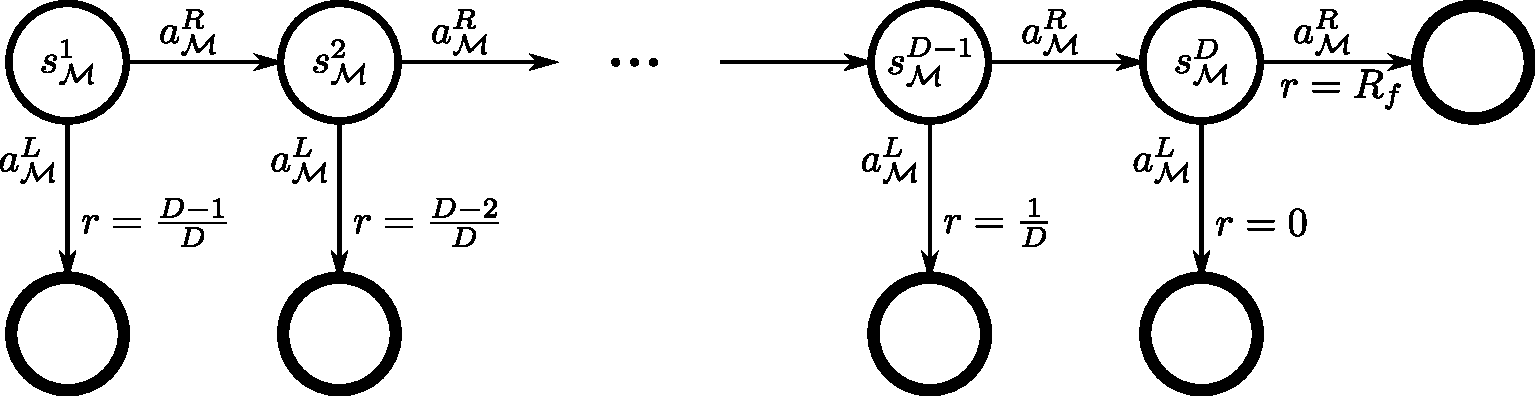
\includegraphics[width=\textwidth]{figures/ch4/mod_dchain_mdp.pdf}
            \caption[An illustration of the \textit{(modified) D-chain problem}.]{An illustration of the \textit{(modified) D-chain problem}, where $\schain{1}$ is the starting state and transitions are deterministic. The reward for taking action $\aR$ from state $\schain{D}$ at the end of the chain is $R_f$, where $R_f=1$ in the original D-chain, and $R_f=\frac{1}{2}$ in the modified D-chain.}
            \label{fig:modified_d_chain}
        \end{figure}

        To intuitively understand why UCT will struggle on this MDP, the reward function can be decomposed into a dense and sparse component:
        \begin{align}
            R_{\dense}(\schain{i},\aL) &= \frac{D-i}{D}, \\
            R_{\dense}(\schain{i},\aR) &= 0, \\
            R_{\sparse}(\schain{i},a) &= \one[i=D] \cdot \one[a=\aR], \\
            R(s,a) &= R_{\dense}(s,a) + R_{\sparse}(s,a).
        \end{align}

        The two components of the rewards can be seen to encourage the agent to perform two different behaviours. In English, the reward $R_{\dense}$ is telling the agent to ``leave the chain as soon as possible and collect a reward as soon as possible'', whereas the sparse reward $R_{\sparse}$ is telling the agent to ``stay on the chain until the end''. As UCT tries to interleve exploration and exploitation, UCT will take the immediate reward of $\frac{D-1}{D}$ on most trials, rather than exploring to find the reward of one. 

        Compounded on this, once a trial of UCT finally reaches the unit reward for the first time, the value estimates of $\Vuct(\schain{i})$ still need many more trials to reach the unit reward for the values to become close to accurate. \citet{dchain} make these arguments more formally to prove that UCT will suffer a regret of $\Omega((\exp \circ \exp \circ ... \circ \exp)(1))$, where $\circ$ denotes functional composition, and there are $D$ many composed exponential functions.

        While from the lens of practical (single-objective) reinforcement the issue may seem like one of poor reward engineering, rewards with conflicting objectives similar to this will naturally arise in the context of multi-objective reinforcement learning. An example of this will be seen in the \textit{Deep Sea Treasure} problem in Chapter \ref{ch:5-chmcts}. \todo{Here I'm referencing that in deep sea treasure, the scalarised reward can be written as} $R=w\cdot R_{\text{time}} + (1-w) R_{\text{treasure}}$, \todo{and its very similar in form to my above decomposition.}

        Introducing entropy as an exploration bonus in this problem helps to solve the problem easily. Once the agent leaves the chain, it can no longer collect an bonus entropy reward, encouraging it to explore down the chain. As can be seen in Figure \ref{fig:d_chain_results}, the D-chain problem is an example of an MDP where the standard and maximum-entropy objectives are well aligned.

        To highlight that in maximum entropy methods that the temperature parameter needs to be tuned precisely per MDP, consider the \textit{modified D-chain problem}, where the sparse reward at the end of the chain is replaced with $R(\schain{D},\aR)=\frac{1}{2}$. In this case the optimal policy takes the immediate reward of $\frac{D-1}{D}$ from the initial state, and the maximum entropy objective is misaligned with the standard objective. \todo{Comment about results}

        \begin{figure}
            \centering
            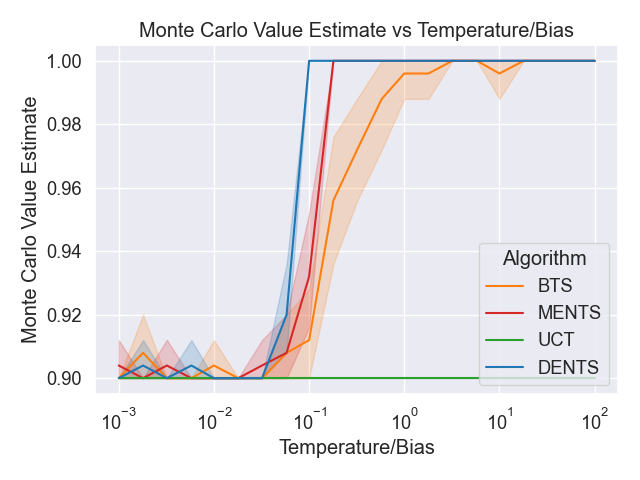
\includegraphics[width=0.49\textwidth]{figures/ch4/ten_chain.png}
            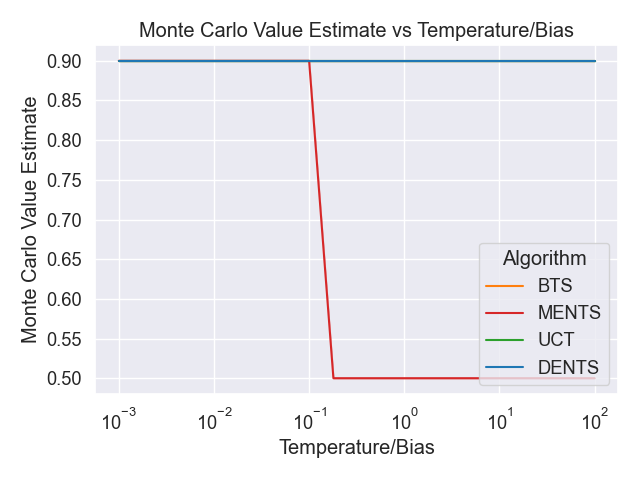
\includegraphics[width=0.49\textwidth]{figures/ch4/mod_ten_chain.png}
            \caption[Results on the (modified) D-chain problem.]{Results on the D-chain problem (left), and the modified D-chain problem (right), for a variety of parameters and with $D=10$. Each algorithm was run for 5000 trials, and results are averaged over 25 repeated experiments. For BTS the temperature function is set to a constant value, and in DENTS the temperature function and entropy weighting function are set to the same constant value. \todo{Make yaxis go from 0 to 1, and add some markers again to make things clearer with overlapping lines.}}
            \label{fig:d_chain_results}
        \end{figure}




    \subsection{The Entropy Trap}

        In the \textit{D-chain with Entropy Trap problem}, or \textit{Entropy Trap problem} for short, an additional chain of states is added to end of the original D-chain to throw off maximum entropy agents. Now at the end of the D-chain, or the \textit{UCT Gauntlet}, the agent has to make a final choice. It can either collect the final sparse reward of one, or it can fall into the \textit{Entropy Trap}, a chain of length $E$, where zero reward is given, but the agent can collect an entropy bonus of up to $E\log(2)$. The Entropy Trap problem is depicted in Figure \ref{fig:entropy_trap}. 

        \htodo{Make proofs use consistent E notation instead of H}

        \begin{figure}
            \centering
            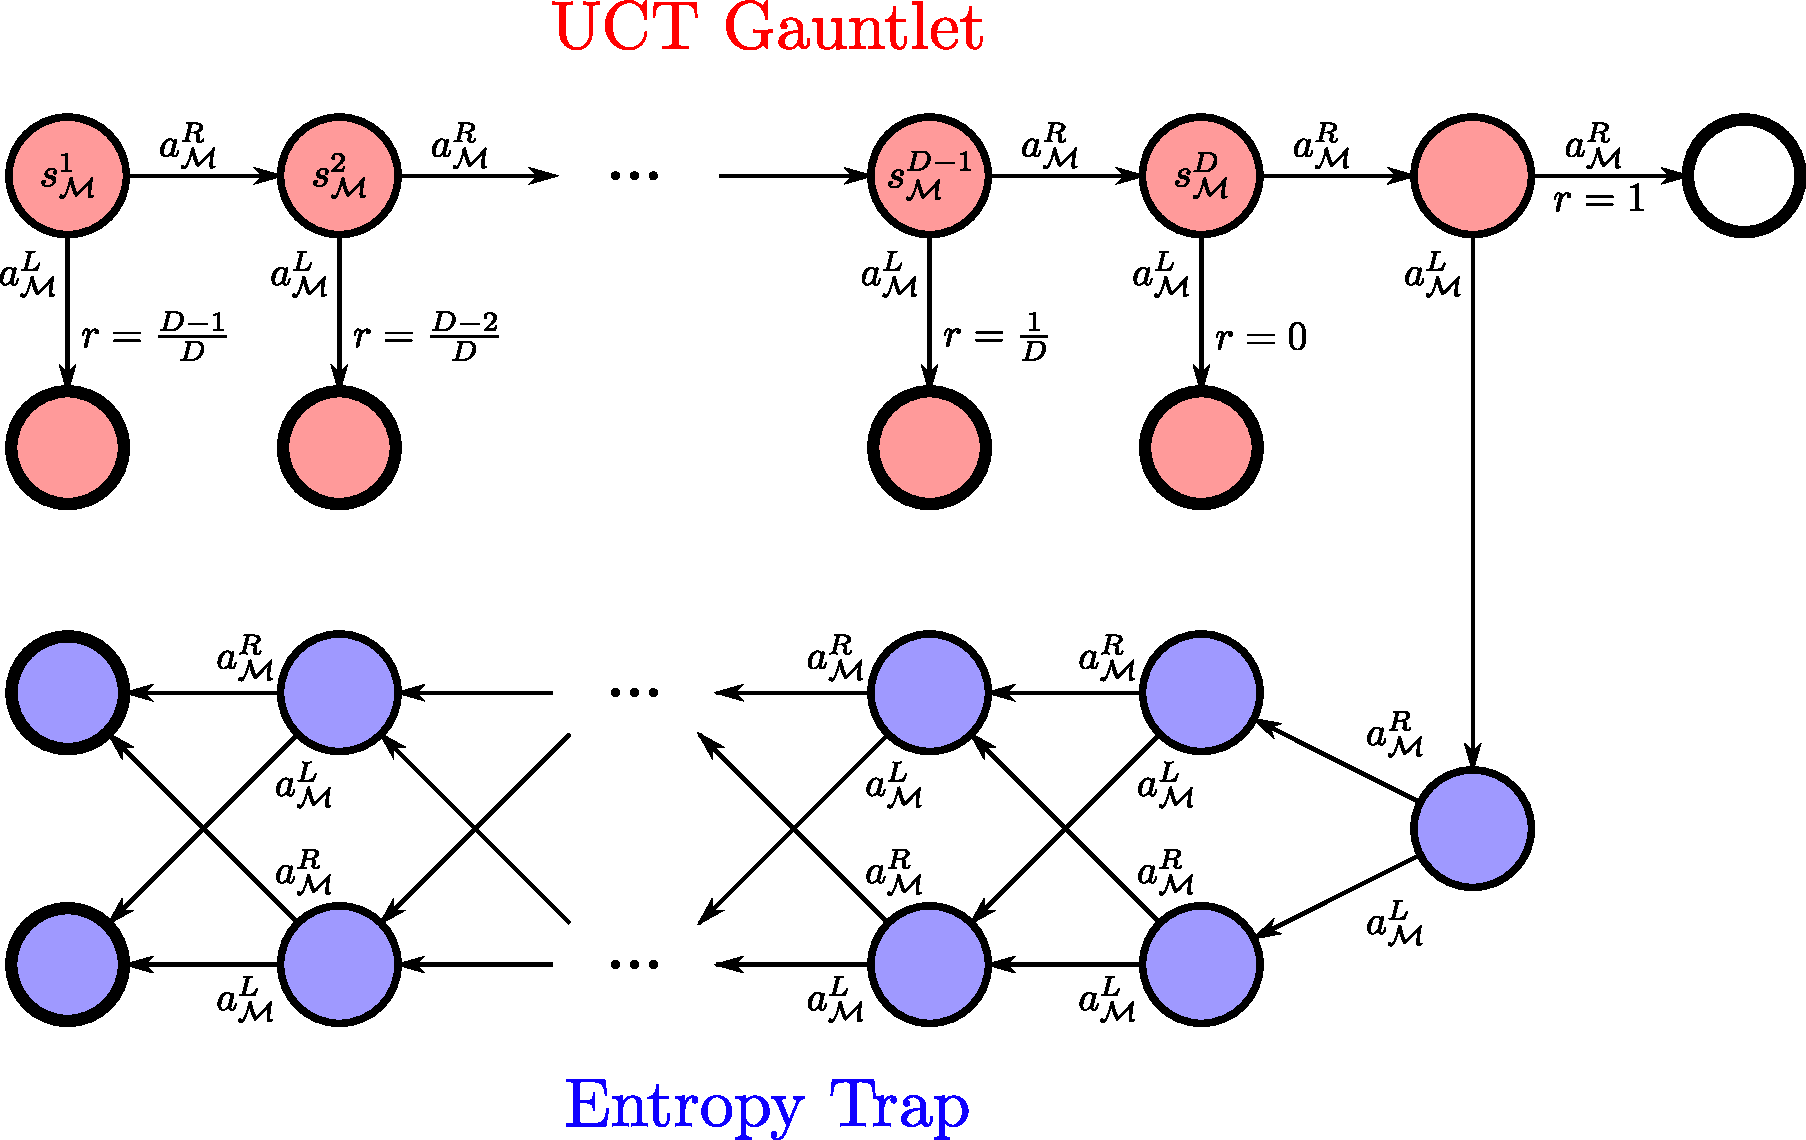
\includegraphics[width=\textwidth]{figures/ch4/entropy_trap_mdp_colour.pdf}
            \caption[An illustration of the \textit{Entropy Trap problem}.]{An illustration of the \textit{Entropy Trap problem}. In red, the original D-chain problem (Figure \ref{fig:modified_d_chain}) is labelled as the UCT Gauntlet, and the additional states added for the Entropy Trap are in blue. If a reward is not specified for a transition it is zero.}
            \label{fig:entropy_trap}
        \end{figure}

        When using the maximum entropy objective, with temperature $\alpha$, in the Entropy Trap problem, an agent can gain an entropy bonus of $\alpha E \log(2)$ from falling in the Entropy Trap. And hence, if $\alpha > \frac{1}{E\log(2)}$, the maximum entropy objective must be misaligned with the standard objective, as the entropy agent can gain an entropy bonus of greater than one from the Entropy Trap. So a maximum entropy agent can be restricted to using an arbitrarily small temperature, by increasing the value of $E$. By setting $D=E$ it can be shown that expectation MENTS will need exponentially many trials with respect to the size of the MDP state space to find the optimal policy: 
        %
        \begin{theorem} \label{thrm:ments_fail}
            There exists an MDP such that MENTS (for any value of $\alphaments$) is either not consistent, or requires an exponential number of trials in the size of the state space. That is, either $\mathbb{E}\sreg(s_0,\psiments)\not\rightarrow 0$ or there exists constants $c,k>0$ such that $\mathbb{E}\sreg(s_0,\psiments) \geq c(1 - \frac{n}{k^{|\cl{S}|}})$. The latter case implies that $\mathbb{E}\sreg(s_0,\psiments)>0$ and $\psiments\neq\pi^*$ for $n<k^{|\cl{S}|}$. 
        \end{theorem}

        Results on the Entropy Trap problem are given for $D=E=10$ and $D=E=15$ in Figure \ref{fig:entropy_trap_results}. When using $D=E=15$ it is feasible that BTS can make progress given enough trials, but ultimately if $D$ is made large enough BTS will also struggle on this environment, as it can only explore randomly. As the likeliehood of reaching the end of the chain through random exploration becomes exponentially less likely, only DENTS is able to solve the Entropy Trap in a reasonable amount of time as $D=E$ is made larger.

        \begin{figure}
            \centering
            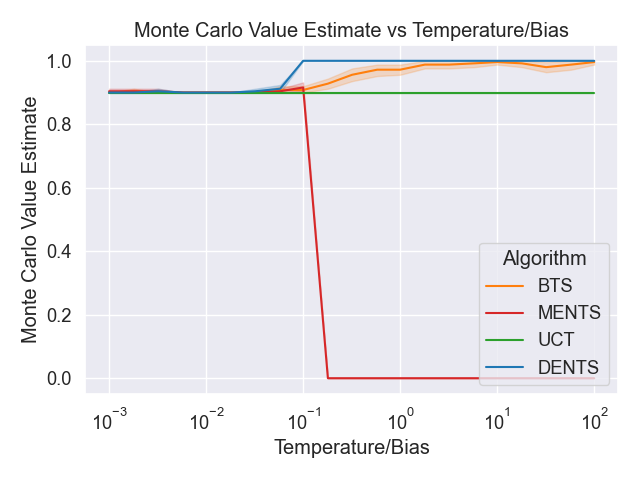
\includegraphics[width=0.49\textwidth]{figures/ch4/entropy_trap_10.png}
            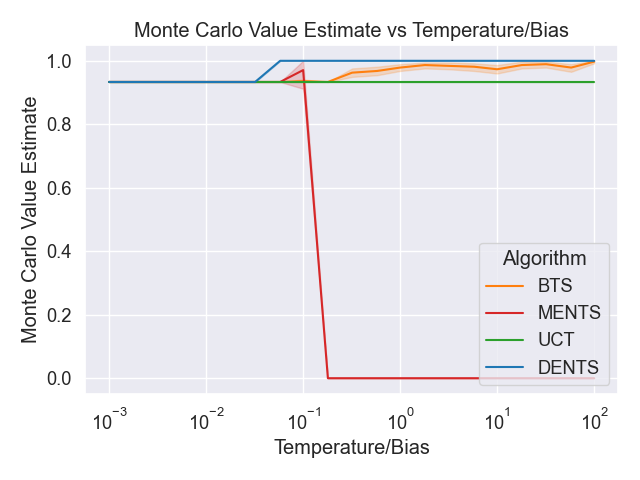
\includegraphics[width=0.49\textwidth]{figures/ch4/entropy_trap_15.png}
            \caption[Results on the Entropy Trap problem.]{Results on the Entropy Trap problem, with $D=E=10$ (left) and $D=E=15$ (right). Each algorithm was run with a variety of temperature/bias parameters, and results are averaged over 25 repeated experiments. In the $D=E=10$ case, each algorithm was run for $5000$ trials, and in the $D=E=15$ case each algorithm was run for $100000$ trials. For BTS the temperature function is set to a constant value, and in DENTS the temperature function and entropy weighting function are set to the same constant value. \htodo{Update thtspp aux to run DENTS with fewer trials, just to show off DENTS a even more.} \htodo{also fiddle with num trials to show things off more. Maybe use 20, for the second plot and let temperatures rise to one order of magnitude more, or lower the number of trials. Basically want the second plot for MENTS to show no progress. First plot increase number of trials until MENTS is just about able to solve it.}}
            \label{fig:entropy_trap_results}
        \end{figure}
        
















    \htodo{below this in tex is original writing about D-chain from NeurIPS. Should make sure that there's no info want to also cover missed in the above. Just re-wrote this section as the arguments are updated and better now.}

    % This section discusses theoretical MDPs, building on top of the intuitions from Section \ref{sec:4-1-intro} to take advantage of the pitfalls of UCT and MENTS. These MDPs can then be used to constructively prove theoretical results. 



    % \todo{Sometimes feel like I'm bashing on MENTS. Want to make it clearer that I'm not bashing on MENTS, but using MENTS (as the max entropy MCTS method) to demonstrate issues with the max entropy objective itself.}

    % This subsection uses theoretical MDPs to further highlight and discuss the benefits and pitfalls of UCT and MENTS, \todo{and compares the performance of BTS and DENTS on these MDPs.} 

    % The \textit{D-chain problem} introduced by \todo{cite} (Figure \ref{fig:modified_d_chain}), is a deterministic MDP for which \todo{UCT ``struggles'' (find better words, maybe here say that wont feasibly solve)}. From some state $d$ if the action $a_L$ is taken the trial ends and a reward of $(D-d)/D$ is received, and from the final state in the chain, $D$, if the action $a_R$ is taken then the maximum reward of $R_f=1$ is received. Hence, the optimal standard policy will always take action $a_R$ at every state achieve a return of $1$.

    % \todo{cite} show that UCT requires $\Omega(\exp(...\exp(1)...))$ many trials (D composed exponential functions) to recommend the optimal actions $a_R$. \bd{Informally, this behaviour stems from the value estimate of state 2 remaining below D-1/D for a long time, and UCT repeatedly taking action aL on its trials once its confidence intervals become relatively concentrated. UCT will still always explore the aR action and eventually converge to the optimal value estimates (and recommendation policy), but in practise it would take longer than a human lifetime.}

    % Where in Section \todo{ref} UCT can be seen to perform well in the presence of an informative dense reward, and struggle when only given an uninformative sparse reward, this MDP sets the rewards to take advantage of this \bd{behaviour maximally. The MDPs rewards can be viewed from the perspective of the dense rewards along the chain that essentially suggest ``don't explore this way'', which are hiding the sparse reward of one at the end of the chain.}

    % In stark contrast, when MENTS is run on the D-chain problem, it quickly explores and finds the sparse reward of one at the end of the chain. This is largely because of the maximum entropy objective, where there \bd{is no entropy reward to be gained by traversing to a sink state, thus encouraging MENTS to follow the chain}. However, because the chain is explored largely due to the maximum entropy objective, consider what happens in the \textit{modified D-chain problem}, where the reward at the end of the chain is set to $R_f=1/2$. \todo{copy out the soft Q value computations with temp of one.}

    % These two cases $R_f \in {1/2,1}$ demonstrate that MENTS, and more generally whenever using the maximum entropy objective, the optimal temperature parameter to be used is dependent on the MDP, and can vary massively even with small changes in the MDP, as for example in this the value of a single reward was changed. \todo{Reference the result that for any temperature there is an MDP where MENTS will be inconsistent}

    % \todo{Generally write up a bit cleaner once have plots in}

    % BTS and DENTS improve on this theoretically as convergence can be guarunteed by parameter settings which are independent of the MDP. In practise, for example consider using a constant value for $\alphadents$ and $\betadents$, the search policy can behave similarly to MENTS, \bd{which could be an issue in more complex MDPs} \todo{some of this discussion more appropriate for entropy trap bit maybe?}



    % \todo{plots to add: the two plots from neurips, performance of MENTS/BTS/DENTS for varying settings of temperature parameters. Same plots for entropy trap D-chain. Also demonstrate that if temperatures decayed properly then DENTS will visit the optimal sink state in entropy D-chain lots, while if not decayed, then will recommend the correct thing, but not visit. Last one is of practical importance, where the sparse reward of one at the end isn't just a sink state but the rest of the MDP where you actually want to do something important.}


    % \bd{(Commented out old writing below this). It is often argued in the maximum entropy objective that the standard objective can be recovered by setting the temperature suffficiently small, however this looses the benefits of using entropy for exploration.} \todo{Ref the result about ments converging for a sufficiently small temperature here.}
    % % In the maximum entropy objective, it is argued that the standard objective can be recovered by setting $\alpha=0$ or setting $\alpha$ infitesimally small ($0<\alpha<<1$). \todo{add quote}. 
    % % %
    % % \todo{Although this is theoretically true (TODO ref the result about MENTS), in practise it is desirable to use the largest temperature that doesn't lead to undesirable (random) behaviour. In other words, extermely small temperatures do not utilise entropy for exploration effectively, while extremely large temperatures encourage agents to act randomly rather (reword: optimise for the standard objective). MENTS is used in (TODO) to demonstrate this issue with the maximum-entropy objective empirically, and (TODO) provides a corresponding theoretical result around MENTS.}
    % % %
    % % Although this is true, the most benefit can be gained from using entropy as an exploration bonus by setting a larger value of $\alpha$. This is highlighted in Figure \todo{ref}, where the performance on MENTS on the modified D-chain environment can be seen to improve as $\alpha$ is made larger, until a sudden drop off when it surpasses a threshold (\todo{at the poing 0.142ish}).


    % By making this observation that maximum entropy algorithms can be mislead by providing an opportunity to accrue the `entropy reward', the D-chain problem can be further adapted, such that neither UCT or MENTS will perform well for any parameter settings. To construct the \textit{D-chain with entropy trap} \bd{problem? MDP?}, the same chain of length $D$, or the \textit{UCT gauntlet}, is used from the D-chain problem, and as such UCT will also struggle on this problem. However, at the end of the chain this time, one more choice is left, to either take the immediate reward of one, or to enter the \textit{entropy trap}, which is a sequence of states with zero rewards that allows a policy to act randomly to gain an entropy reward.
    % %
    % \begin{figure}
    %     \centering
    %     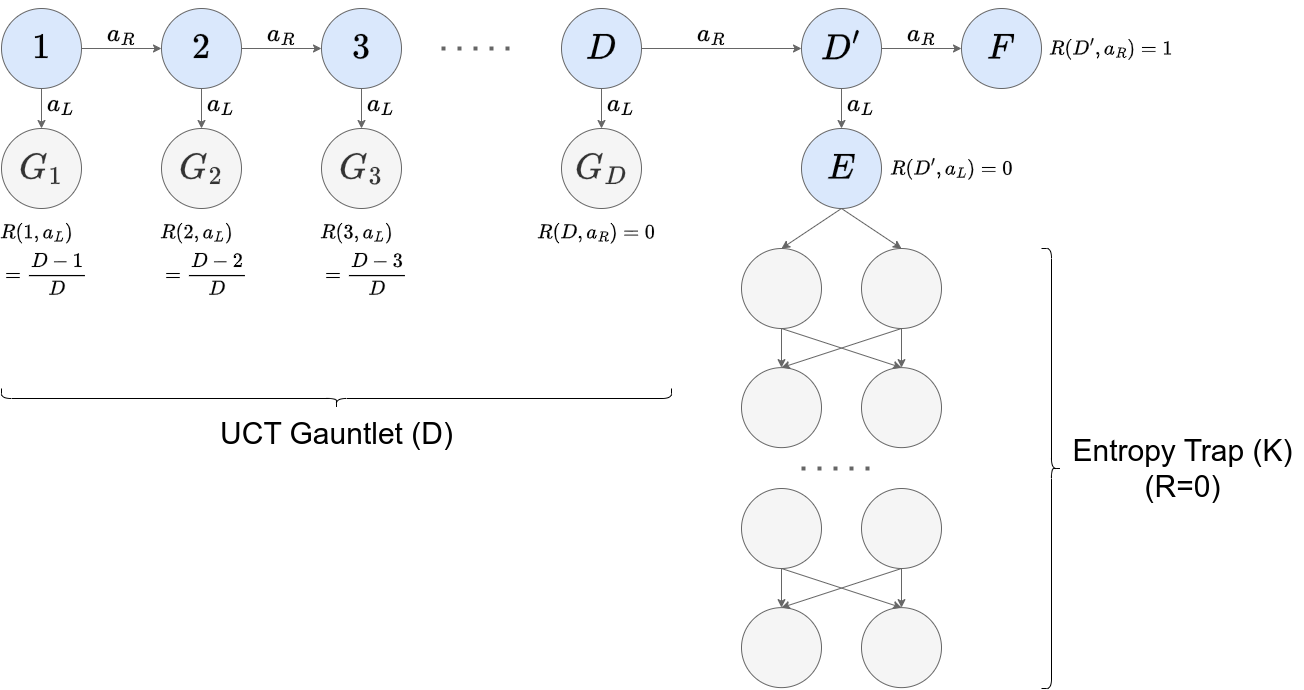
\includegraphics[width=0.6\textwidth]{figures/temp/entropy_trap.png}
    %     \caption[An illustration of the \textit{(modified) D-chain problem with entropy trap}.]{An illustration of the \textit{(modified) D-chain problem with entropy trap}, \todo{write caption describing MDP after made it}. \todo{Temp fig}}
    %     \label{fig:d_chain_entropy_trap}
    % \end{figure}

    % \todo{These claims made more concrete in (ref theorem)}

    % \todo{Some writing about what the plots show empirically once run this.}

    % \todo{Wrap up this section saying that although these are highly theoretical and constructed examples, it can help even in practise to think about these things and consider the performance on these envs to understand why these algorithms behave the way they do on real problems. For example, it may be the case that there are some subtle entropy traps, consider if instead that Rf was 10, and the entropy trap had a reward of 9 (including the entropy bit), such that the performance looked good but } \todo{Basically a bit of chatting to map back to these things in practise and why useful, maybe also add something like this at the top. Actually, add this at the top, and then point out the specifics at the end. Good sandwitch storytelling.}

    % \todo{Below is parameter sensitivity section from neurips appendix D. Extract whats useful, but better results should demonstrate this better}

    % We run each algorithm with a variety of $\alpha$ temperatures, and the $\epsilon$ exploration parameter on the 10-chain environments (Figure \ref{fig:dchain_illustration}). Additionally, we ran UCT with a variety of bias parameters. Figures \ref{fig:uct_10chain_hps}, \ref{fig:ments_10chain_hps}, \ref{fig:rents_10chain_hps}, \ref{fig:tents_10chain_hps}, \ref{fig:bts_10chain_hps} and \ref{fig:dents_10chain_hps} give results for the 10-chain environment, with algorithms UCT, MENTS, RENTS, TENTS, BTS and DENTS respectively. Figures \ref{fig:uct_10chain_half_hps}, \ref{fig:ments_10chain_half_hps}, \ref{fig:rents_10chain_half_hps}, \ref{fig:tents_10chain_half_hps}, \ref{fig:bts_10chain_half_hps} and \ref{fig:dents_10chain_half_hps} give results for the modified 10-chain environment, with algorithms UCT, MENTS, RENTS, TENTS, BTS and DENTS respectively. 

    % As expected with UCT, regardless of how the bias parameter is set, in both the 10-chain ($D=10$, $R_f=1.0$) and modified 10-chain ($D=10$, $R_f=0.5$) environments, it only achieves a value of $0.9$. See Figures \ref{fig:uct_10chain_hps} and \ref{fig:uct_10chain_half_hps} for plots.

    % As discussed in Section \ref{sec:limitations}, for higher temperatures in MENTS it will find the reward of $R_f$ in both the 10-chain and modified 10-chain environments. At a temperature of $\alpha=0.15$ MENTS is able to find the reward of $R_f=1$ on the 10-chain (Figure \ref{fig:ments_10chain_hps}), but will still recommend a policy that gives the reward of $R_f=0.5$ on the modified 10-chain (Figure \ref{fig:ments_10chain_half_hps}). At a temperature of $\alpha=0.1$ MENTS will struggle to find the reward of $R_f=1$ in the 10-chain, without the help of the exploration parameter, but this is the first temperature we tried that was able to recommend the optimal policy in the modified 10-chain (Figure \ref{fig:ments_10chain_half_hps}). For low temperatures, such as $\alpha=0.01$, MENTS was able to find the optimal policy, but in the case of the 10-chain with $R_f=1$ it can only do so with the help of a higher exploration parameter.

    % When we ran TENTS on the (modified) 10-chain, we see results that parallel MENTS, see Figures \ref{fig:tents_10chain_hps} and \ref{fig:tents_10chain_half_hps}. Interestingly, RENTS was only able to find the reward of $R_f=1$ on the 10-chain environment if we used a low temperature, $\alpha=0.01$ and a high exploration parameter, $\epsilon=10$. Otherwise, RENTS tended to behave similarly to UCT on these environments, see Figures \ref{fig:rents_10chain_hps} and \ref{fig:rents_10chain_half_hps}.

    % In contrast, BTS was able to find the reward of $R_f=1.0$ in the 10-chain when a high search temperature or high exploration parameter was used (Figure \ref{fig:bts_10chain_hps}). And, in the modified 10-chain, BTS always achieves a reward of $0.9$ regardless of how the parameters are set (Figure \ref{fig:bts_10chain_half_hps}). DENTS performance on the 10-chain (Figure \ref{fig:dents_10chain_hps}) and modified 10-chain (Figure \ref{fig:dents_10chain_half_hps}) was similar to BTS, but tended to find the reward of $R_f=1$ in the 10-chain marginally faster. For the decay function $\beta$ in DENTS, we always set $\beta(m)=\alpha/\log(e+m)$ for these experiments.

    % To demonstrate that the $\epsilon$ exploration parameter is insufficient to make up for a low temperature, we also consider the 20-chain ($D=20$, $R_f=1$) and modified 20-chain ($D=20$, $R_f=0.5$) problems. We don't give plots for all algorithms on both of the 20-chain environments like we do for 10-chain environments, but opt for the plots that demonstrate something interesting. 
    
    % In Figure \ref{fig:ments_20chain_hps} we see MENTS on the 20-chain is able to find the reward of $R_f=1$ for higher temperatures. However, this time, the exploration parameter does not make much of an impact when using lower temperatures. Moreover, a large exploration parameter appears to negatively impact MENTS ability to find $R_f=1$. This makes sense considering that a uniformly random policy will find the reward at the end of the chain once every $2^{10}$ trials in the 10-chain, but only once every $2^{20}$ in the 20-chain. Again, on the modified 20-chain, MENTS is only able to recommend the optimal policy for low temperatures (see Figure \ref{fig:ments_20chain_half_hps}). 

    % When we ran BTS on the 20-chain, it was unsuccessful at finding the final reward of $R_f=1$, which makes sense as it is not using entropy for exploration, and it is unlikely to follow a random policy to the end of the chain (Figure \ref{fig:bts_20chain_hps}). For DENTS, we again used a decay function of $\beta(m)=\alpha/\log(e+m)$ for simplicity, and unfortunately it was only able to make slow progress towards finding the final reward of $R_f=1$ for high temperatures. However, if we independently set the values of $\alpha$ and 
    
    % However, DENTS on the 20-chain begins to make slow progress towards finding the final reward of $R_f=1$, but requires a higher temperature to be used, as we decay the weighting of entropy over time (Figure \ref{fig:dents_20chain_hps}). Again we used a decay function of $\beta(m)=\alpha/\log(e+m)$ here for simplicity, and if we properly select them DENTS is more than capable of solving the 20-chain. For example we show that using DENTS with $\alpha=0.5$, $\beta(m)=10/\log(e+m)$ and $\epsilon=0.01$ in Figure \ref{fig:dents_20chain_tuned}, where $\alpha$ is set low enough that there is still a high probability of following the chain to the end, $\beta$ is set to be large initially to encourage exploring with the entropy reward and $\epsilon$ is set low to avoid random exploration ending trials before reaching the end of the chain. If we were to run DENTS and BTS on the modified 20-chain they would recommend the optimal policy giving a value of $0.95$ for all of the parameters we searched over (not shown).
    
    % Finally, in Figure \ref{fig:dbments_20chain_hps} we also consider running DENTS, but instead setting $\beta(m)=\alpha$ to replicate MENTS. The main difference between DENTS in this case and MENTS is the recommendation policy, where DENTS uses the Bellman values for recommendations, rather than soft values. So even in cases where the MENTS search is more desirable, we can replicate it with DENTS while providing recommendations for the standard objective. Moreover, running DENTS with $\beta(m)=\alpha$ on the modified 20-chain would always yield the optimal value of $0.95$ because of the use of Bellman values for recommendations (not shown).


    % \todo{A MILLION FIGURES WERE HERE}











\section{Empirical Results}
\label{sec:4-4-results}
    
    \htodo{Wasn't too careful about changing from active voice to passive voice here in this entire section}

    \htodo{Get some better results using hyperparam optimise //// want a dense env where the (not entropy) temp decay fn gets optimised to soemthing that decays a lot /// want a sparse env where the temp decay fn gets optimised to something flat (or basically flat)}

    This section provides empirical results on gridworld environments and on the game of Go. It begins by describing the environments, the evaluation setup, and is followed by the empirical results and discussion. The main algorithms discussed in this chapter, BTS and DENTS will be evaluated, using UCT, MENTS, RENTS, TENTS and H-MCTS as baselines \htodo{ref litrev or cite?}. 




    \subsection{Environments}

        \subsubsection{(Deterministic) Frozen Lake}
            The \emph{(Deterministic) Frozen Lake} \htodo{remove deterministic} is a grid world environment with one goal state. The agent can move in any cardinal direction at each time step, and walking into a wall leaves the agent in the same location. \htodo{Add is slippery description.} Trap states exist where the agent falls into a hole and the trial ends. \htodo{remove next sentence and add paragraph below.} If the agent arrives at the goal state after $t$ timesteps, then a sparse reward of $0.99^t$ is received. \htodo{Also add dense reward -1, remove the determinsitic bit, and describe the is slippery option too.}

            \htodo{Two rewards considered. Dense uninformative reward of -1 everywhere, and when falling in a hole the agent gets stuck and recieves a total return of -H. Second reward is sparse, where agents gets a reward of one for reaching the goal state. When is slippery is not on, a discount factor is used, so that shorter paths gain more reward than longer ones. This can effectively be implemented by returning gamma to the t in the deterministic case when agent reaches goal after t timesteps.}

            \htodo{ Extra credit: would like to have experiments which vary the proportion of the sparse reward. So have FL(lambda), where lambda specifies the ratio between the dense and sparse rewards. Then investigate what happens as vary lambda. So this is the grid world experiments run again, }

            Figure \ref{fig:fl_maps} gives the specific maps used for Frozen Lake in these experiments. In the maps, \texttt{S} denotes the starting location of the agent, \texttt{F} denotes spaces the agent can move to, \texttt{H} denote holes that end the agents trial and \texttt{G} is the goal location. 

            An 8x8 map (Figure \ref{fig:fl8}) is used in Section \ref{sec:param_sens_fl} to demonstrate how the different Boltzmann search and entropy based algorithms perform with a variety of temperature parameters. The 8x12 map (Figure \ref{fig:fl12}) is used for an environment that is sufficiently large map to test and compare algorithms. Each of these maps was randomly generated, with each location having a probability of $1/5$ of being a hole, and the maps were checked to have a viable path from the starting location to the goal location. \htodo{with the exception of maps XXX, YYY, which were not randomly generated for these experiments, and chosen to correspond to the default maps for that size in Gymnasium (TODO: cite)}
        
            \begin{figure}
                \centering
                \begin{subfigure}[b]{0.3\textwidth}
                    \centering
                    \texttt{SFFFFFHF} \\
                    \texttt{FFFFFFFF} \\
                    \texttt{FHFHFFFF} \\
                    \texttt{FFFFFFHH} \\
                    \texttt{FFFHFFFF} \\
                    \texttt{FHHHFFFF} \\
                    \texttt{FFFFFHFF} \\
                    \texttt{FFFFFFFG} 
                    \caption{8x8 Frozen Lake.}
                    \label{fig:fl8}
                \end{subfigure}
                % \hfill
                \begin{subfigure}[b]{0.3\textwidth}
                    \centering
                    \texttt{SFHFFFHFFFFF} \\
                    \texttt{FFFFFFFHFFFF} \\
                    \texttt{HFFFFFHFFFFF} \\
                    \texttt{FHFFHFFFFFFF} \\
                    \texttt{HHFFFFFFFFFF} \\
                    \texttt{FHFFFFHFFFFF} \\
                    \texttt{FHFFFHHFHFFF} \\
                    \texttt{FFFFFFFFFHHG} 
                    \caption{8x12 Frozen Lake.}
                    \label{fig:fl12}
                \end{subfigure}
                % \hfill
                % \begin{subfigure}[b]{0.3\textwidth}
                %     \centering
                %     \texttt{SFHFFFFFFFHF} \\
                %     \texttt{FFFFFFFFFFFF} \\
                %     \texttt{FHFFFFHFFFFF} \\
                %     \texttt{FFFHFFFFFFHF} \\
                %     \texttt{FFFFFFFFFFFF} \\
                %     \texttt{FFFFHFFFHFFF} \\
                %     \texttt{FFHFFFFFFFFH} \\
                %     \texttt{FFFFFFFFFFFG} 
                %     \caption{8x12 Test Frozen Lake.}
                %     \label{fig:fl12test}
                % \end{subfigure}
                \caption[Maps used for the Frozen Lake environment.]{Maps used for the Frozen Lake environment. \texttt{S} is the starting location for the agent, \texttt{F} represents floor that the agent can move too, \texttt{H} are holes that end the agents trial and \texttt{G} is the goal location. \htodo{Add 4x4, 5x5 or 4x6, 6x6 or 4x8 maps for stoch envs} \htodo{Add 8x8, 8x12 or 8x16, 12x12 or 16x16 maps} \htodo{use standard maps from gym where possible}}
                \label{fig:fl_maps}
            \end{figure}




        \subsubsection{Sailing Problem}
            The \emph{Sailing Problem} is another grid world environment with one goal state, at the opposite corner to the starting location of the agent. This problem has often been used to evaluate MCTS algorithms \cite{peret2004line,uct,tolpin2012mcts,brue1}. 
            
            The agent has 8 different actions, where it can travel in any cardinal or semi-cardinal direction. In each state of the MDP, the wind is blowing in a given direction and will stochastically change after every transition. The agent cannot sail directly into the wind. Actions and wind directions can take values in $\{0,1,...,7\}$, with a value of $0$ representing North/up, $2$ representing East/right, $4$ representing South/down and $6$ representing West/right. The remaining numbers represent the inter-cardinal directions. The cost of each action depends on the \textit{tack}, the angle between the direction of the agent's travel and the wind. \htodo{The agent incurs a (dense) cost of (thetawind - theta)/45 + 1 for traveling at angle theta when wind is in direction thetawind.}

            Figure \ref{fig:sailing_deets} gives the map and wind transition probabilities for the Sailing problem, using the same map notation as for Frozen Lake. 

            \begin{figure}
                \centering
                \begin{subfigure}[b]{0.49\textwidth}
                    \centering
                    \texttt{FFFFFG} \\
                    \texttt{FFFFFF} \\
                    \texttt{FFFFFF} \\
                    \texttt{FFFFFF} \\
                    \texttt{FFFFFF} \\
                    \texttt{SFFFFF} 
                    \caption{6x6 Sailing Problem map.}
                \end{subfigure}
                % \hfill
                \begin{subfigure}[b]{0.49\textwidth}
                    \centering
                    \begin{align*}
                        \begin{pmatrix}
                        0.4 & 0.3 & 0.0 & 0.0 & 0.0 & 0.0 & 0.0 & 0.3 \\
                        0.4 & 0.3 & 0.3 & 0.0 & 0.0 & 0.0 & 0.0 & 0.0 \\
                        0.0 & 0.4 & 0.3 & 0.3 & 0.0 & 0.0 & 0.0 & 0.0 \\
                        0.0 & 0.0 & 0.4 & 0.3 & 0.3 & 0.0 & 0.0 & 0.0 \\
                        0.0 & 0.0 & 0.0 & 0.4 & 0.2 & 0.4 & 0.0 & 0.0 \\
                        0.0 & 0.0 & 0.0 & 0.0 & 0.3 & 0.3 & 0.4 & 0.0 \\
                        0.0 & 0.0 & 0.0 & 0.0 & 0.0 & 0.3 & 0.3 & 0.4 \\
                        0.4 & 0.0 & 0.0 & 0.0 & 0.0 & 0.0 & 0.3 & 0.3 
                        \end{pmatrix}
                    \end{align*}
                    \caption{Wind transition probabilities.}
                \end{subfigure}
                \caption[The map and wind transition probabilities used for the 6x6 Sailing Problem.]{The map and wind transition probabilities used for the 6x6 Sailing Problem. The same notation is used for the map as Figure \ref{fig:fl_maps} For the wind transition probabilities, the $(i,j)th$ element of the matrix denotes the probability that the wind changes from direction $i$ to direction $j$, where $0$ denotes North/up, $1$ denotes North-East/up-right, and so on.}
                \label{fig:sailing_deets}
            \end{figure}




        \subsubsection{Go}
            For a more challenging domain, a round-robin tournament was run on the game of Go, which has widely motivated the development of MCTS methods \cite{gelly2007combining,alpha_go,alpha_go_zero}. \textit{Area scoring} is used to score the games, with a \textit{komi} (a score handicap for black) of $7.5$. 
            
            The open-source library KataGo \cite{katago} was used to provide a value network $\tilde{V}$ and prior policy network $\tilde{\pi}$ for the algorithms. 
            
            PUCT algorithm \cite{poly_uct} was used as a baseline algorithm, as described in Alpha Go Zero \cite{alpha_go_zero}, using prioritised UCB \cite{prio_ucb} to utilise the policy neural network. Each algorithm was limited to $5$ seconds of compute time per move, allowed to use $32$ search threads per move, and had access to 80 Intel Xeon E5-2698V4 CPUs clocked at 2.2GHz, and a single Nvidia V100 GPU on a shared compute cluster.

            The methods described in this chapter can be adapted for two-player games by using a discount factor in the MDP. The value of a policy $\pi$ with a discount factor $\gamma$ is defined as:
            \begin{align}
                V^{\pi}(s;t) = \bb{E}_{\tau\sim\pi}\left[\sum_{i=t}^{H-1} \gamma^{i-t}r_i \Bigg| s_t=s \right].
            \end{align}
            %
            \todo{should define this in ch2? It's only really relevant here, and kind of in Frozen lake}
            If the two players are using the policies $\pi_0$ and $\pi_1$, and $\pi$ is the policy that interleves $\pi_0$ at even timesteps with $\pi_1$ at odd timesteps, then using a discount factor of $\gamma=-1$ is sufficient to handle two-player games. \htodo{assuming that the reward function always gives rewards from the perspective of the player taking the current action.}
        
        












    \subsection{Evaluation Proceedure} 

        Consider an algorithm with search tree $\cl{T}$, which provides a partial recommendation policy $\psi_{\text{alg}}$. The recommendation policy is made complete by using a uniformly random policy for states and actions that are outside of the tree $\cl{T}$ as follows:
        % 
        \begin{align}
            \psi(a|s) =
            \begin{cases}
                1                       & \text{ if } s\in\cl{T} \text{ and } a=\psi_{\text{alg}}(s), \\
                0                       & \text{ if } s\in\cl{T} \text{ and } a\neq\psi_{\text{alg}}(s), \\
                \frac{1}{|\cl{A}|}      & \text{ otherwise.}
            \end{cases} \label{eq:full_Recommend}
        \end{align}
        % 
        Using the completed policy $\psi$, a monte carlo value estimate of $V^{\psi}$ is computed by sampling a number of trajectories from $\psi$ and averaging the returns. \htodo{Kind of want a better argument for this line of eval here.} Although this proceedure is evaluating the algorithms in an \textit{offline planning} setting, it still indicates how the algorithms perform in an \textit{online} setting when planning in simulation is interleaved with letting the agent act in the real environment. \htodo{either scrap the evaluation question, or do something more to justify this.But should say something like "this evaluates the policy, and the online performance depends on the policies produced online, therefore correlated"}

        All experiments in this chapter were run with \mctsmode\ewe turned off and did not use the Alias method as described in Section \ref{sec:4-2-3-stoch_search_policies}, apart from the experiments on Go, which used \mctsmode and the Alias method.




        \subsubsection{Gridworld Hyperparameter Selection}

            To select hyperparameters for the algorithms in the gridworld environments, the BayesOpt package \cite{bayesopt} was used. Full details on the hyperparameter tuning and the selected parameters are given in Appendix \ref{appsec:hps}.

            These experiments were run with \mctsmode\ewe turned off and did not use the Alias method (Section \ref{sec:4-2-3-stoch_search_policies}).


            
        \subsubsection{Go Hyperparameter Selection}

            To tune hyperparemters for algorithms used in the Go experiments, a methodical sequence of round robin tournaments were run on a $9\times 9$ board, where in each tournament one parameter was tuned at a time. Full details of these tournaments and the selected hyperparamters are given in Appendix \ref{appsec:go_hps}.

            Of note, both Bellman value estimates and average returns were considered for the Go round robin. In the hyperparamter tuning the two versions of each algorithm were tuned seperately and then played against each other. In each case the average returns algorithms decisively beat the Bellman versions. This could have been because of average returns helping to average out noisy neural network outputs, and the ability of the AR algorithms to run more trials (as described in Section \ref{sec:4-2-3-stoch_search_policies}) in the given search time.
            
            These experiments were run with \mctsmode\ewe turned on and made use of the Alias method (Section \ref{sec:4-2-3-stoch_search_policies}). Additionally, the value network $\tilde{V}$ was used for the value initialisation function $\Vinit$, and prior policy network $\tilde{\pi}$ was mixed into the search policy as described in Section \ref{sec:4-2-3-stoch_search_policies}.

            





    \subsection{Results and Discussion}

        \htodo{Wanted to show the breadth first search if Qinit incorrectly set then get breadth first search in costs case. If can estimate, for example know Rmin and can get Qinit to H times Rmin then can do that. Another zero knowledge Qinit function can use is Qinit equals min a Q(s,a) where for (s,a) in tree, if no such (s,a) then zero (its uniform policy then anyway).}

        \htodo{Talk about how exploitation is useful in two cases in the exploration setting. When have stochastic env, need to exploit to get better value estimates. When env is very large, need exploitation to explore deeper parts of env. Also exploiting helpful when reward is dense and/or informative}

        \htodo{Should also eval AR-BTS etc on these envs? Might make the arguments/results nicer and more complete}

        This subsection first demonstrates the parameter sensitivity of maximum entropy methods on the Frozen Lake environment. Then results on Frozen Lake and the Sailing problem are given with optimised parameters, and finally results from the Go round robin.







        \subsubsection{Parameter sensitivity in Frozen Lake} \label{sec:param_sens_fl}

            \htodo{this subsubsection currently just a c and p from neurips}

            Further discussion on sensitivity to the temperature parameter in MENTS \cite{ments}, RENTS and TENTS \cite{rentsmytents} is now given. Results on the 8x8 Frozen Lake environment (Figure \ref{fig:fl8}) are given using a variety of temperatures to demonstrate how each algorithm performs with different temperatures in that domain. 

            \htodo{clean up hyperparam setting }
            % MENTS, RENTS, TENTS, BTS and DENTS were run with a variety of temperatures on the 8x8 Frozen Lake environment given in Figure \ref{fig:fl8}. Again, we set $\beta(m)=\alpha/\log(e+m)$ for the decay function in DENTS, and we used an exploration parameter of $\epsilon=1$ for all of the algorithms. 

            In Figures \ref{fig:fl_param_sens_ments} and \ref{fig:fl_param_sens_tents} MENTS and TENTS take the scenic route to the goal state for medium temperatures, where the reward for reaching the goal is still significant, but they can obtain more entropy reward by wondering around the gridworld for a while first. For higher temperatures they completely ignore the goal state, opting to rather maximise policy entropy. Interestingly, RENTS in Figure \ref{fig:fl_param_sens_rents} fared better than MENTS and TENTS and never really ignored the goal state for all of the temperatures considered.

            In contrast, both BTS and DENTS were relativly agnostic to the temperature parameter in this environment (with $\epsilon=1$) and were always able to find the goal state. Curves for BTS and DENTS are included in all of Figures \ref{fig:fl_param_sens_ments}, \ref{fig:fl_param_sens_tents} and \ref{fig:fl_param_sens_rents} for reference and as a comparison for MENTS, RENTS and TENTS.
        
            % \FloatBarrier
            
            \begin{figure}
                \centering
                
                \begin{subfigure}[b]{0.32\textwidth}
                    \centering
                    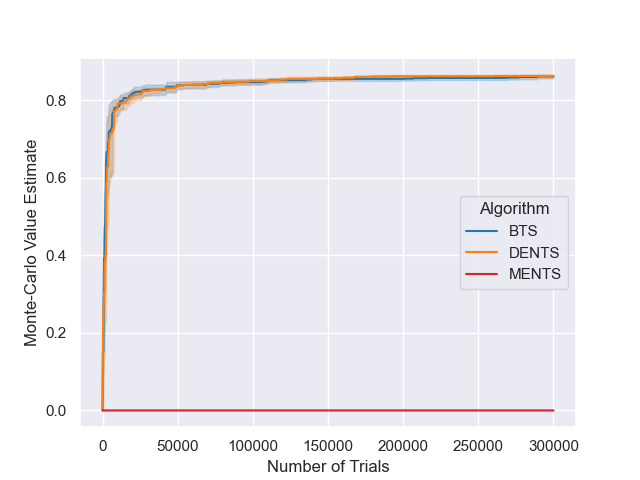
\includegraphics[width=\textwidth]{figures/temp/fl_sens/053_fl8_1_0_01.png}
                    \caption{$\alpha=1$}
                \end{subfigure}
                \begin{subfigure}[b]{0.32\textwidth}
                    \centering
                    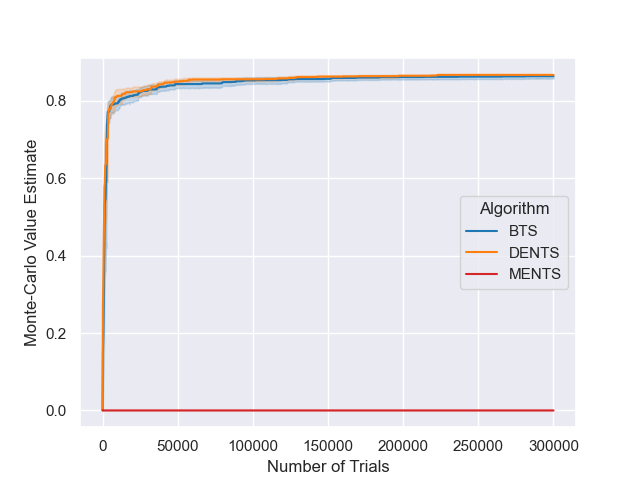
\includegraphics[width=\textwidth]{figures/temp/fl_sens/054_fl8_0_5_01.png}
                    \caption{$\alpha=0.5$}
                \end{subfigure}
                \begin{subfigure}[b]{0.32\textwidth}
                    \centering
                    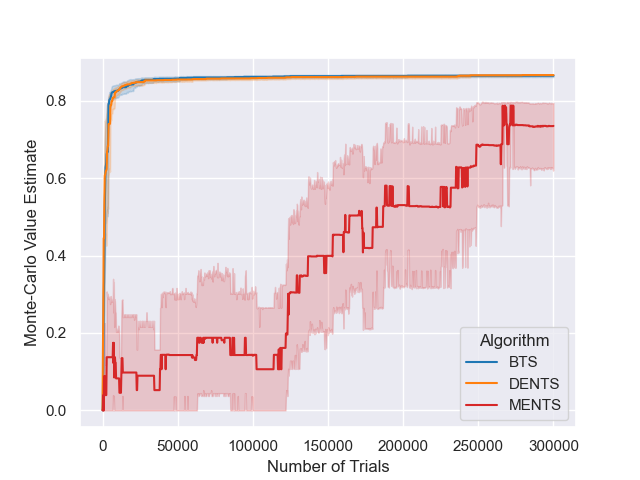
\includegraphics[width=\textwidth]{figures/temp/fl_sens/055_fl8_0_1_01.png}
                    \caption{$\alpha=0.1$}
                \end{subfigure}
                
                \begin{subfigure}[b]{0.32\textwidth}
                    \centering
                    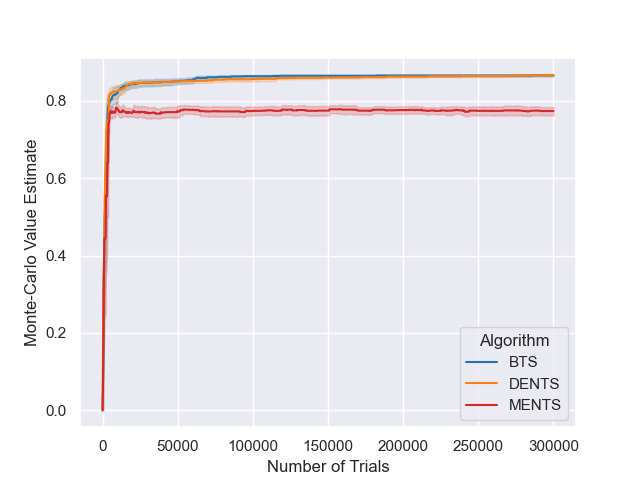
\includegraphics[width=\textwidth]{figures/temp/fl_sens/056_fl8_0_05_01.png}
                    \caption{$\alpha=0.05$}
                \end{subfigure}
                \begin{subfigure}[b]{0.32\textwidth}
                    \centering
                    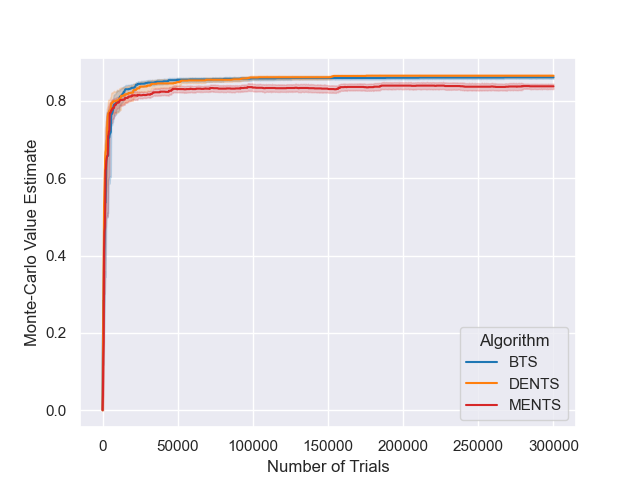
\includegraphics[width=\textwidth]{figures/temp/fl_sens/057_fl8_0_01_01.png}
                    \caption{$\alpha=0.01$}
                \end{subfigure}
                \begin{subfigure}[b]{0.32\textwidth}
                    \centering
                    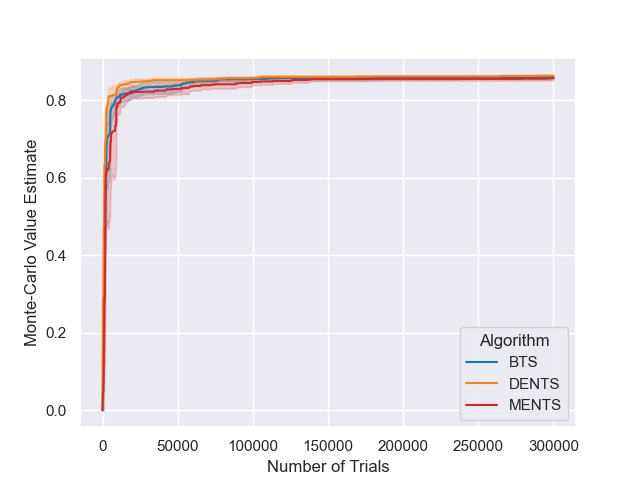
\includegraphics[width=\textwidth]{figures/temp/fl_sens/058_fl8_0_005_01.png}
                    \caption{$\alpha=0.005$}
                \end{subfigure}
                
                \caption{MENTS with a variety of temperatures on an 8x8 Frozen Lake environment. BTS and DENTS are included for reference. \todo{Update fig?}}
                \label{fig:fl_param_sens_ments}
            \end{figure}
            
            \begin{figure}
                \centering
                
                \begin{subfigure}[b]{0.32\textwidth}
                    \centering
                    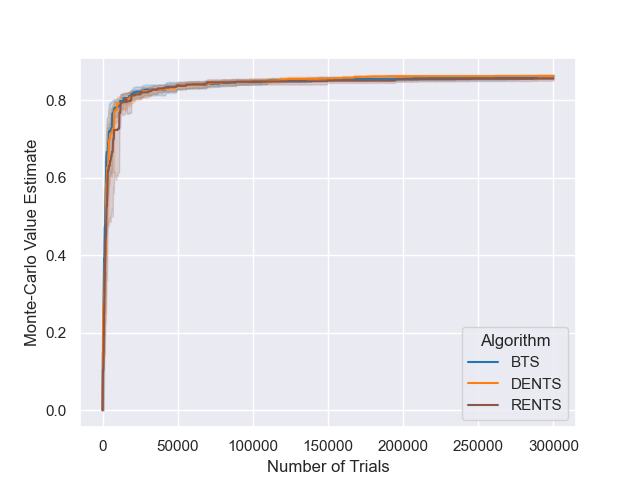
\includegraphics[width=\textwidth]{figures/temp/fl_sens/053_fl8_1_0_02.png}
                    \caption{$\alpha=1$}
                \end{subfigure}
                \begin{subfigure}[b]{0.32\textwidth}
                    \centering
                    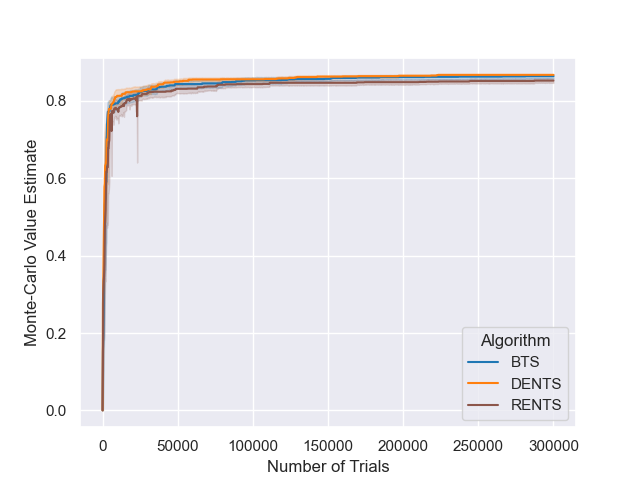
\includegraphics[width=\textwidth]{figures/temp/fl_sens/054_fl8_0_5_02.png}
                    \caption{$\alpha=0.5$}
                \end{subfigure}
                \begin{subfigure}[b]{0.32\textwidth}
                    \centering
                    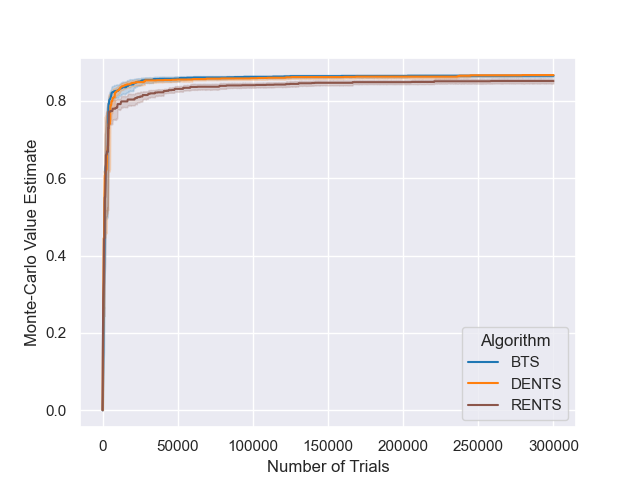
\includegraphics[width=\textwidth]{figures/temp/fl_sens/055_fl8_0_1_02.png}
                    \caption{$\alpha=0.1$}
                \end{subfigure}
                
                \begin{subfigure}[b]{0.32\textwidth}
                    \centering
                    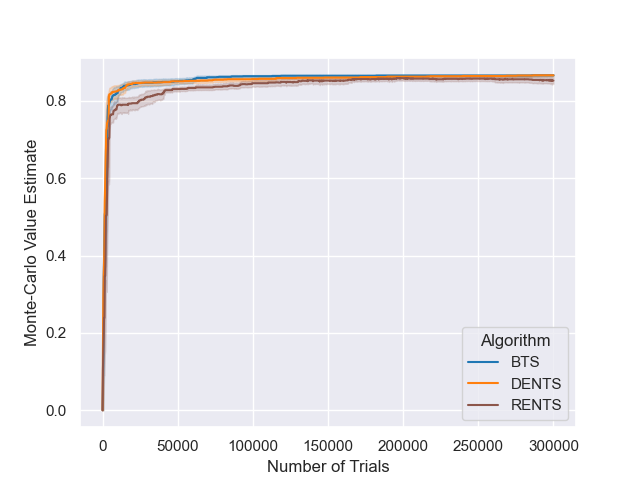
\includegraphics[width=\textwidth]{figures/temp/fl_sens/056_fl8_0_05_02.png}
                    \caption{$\alpha=0.05$}
                \end{subfigure}
                \begin{subfigure}[b]{0.32\textwidth}
                    \centering
                    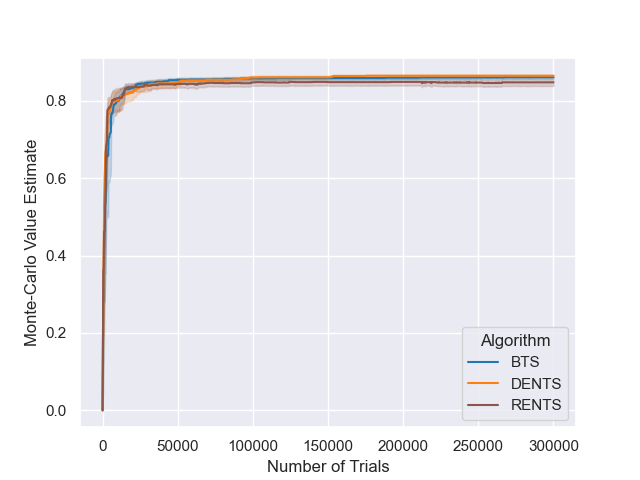
\includegraphics[width=\textwidth]{figures/temp/fl_sens/057_fl8_0_01_02.png}
                    \caption{$\alpha=0.01$}
                \end{subfigure}
                \begin{subfigure}[b]{0.32\textwidth}
                    \centering
                    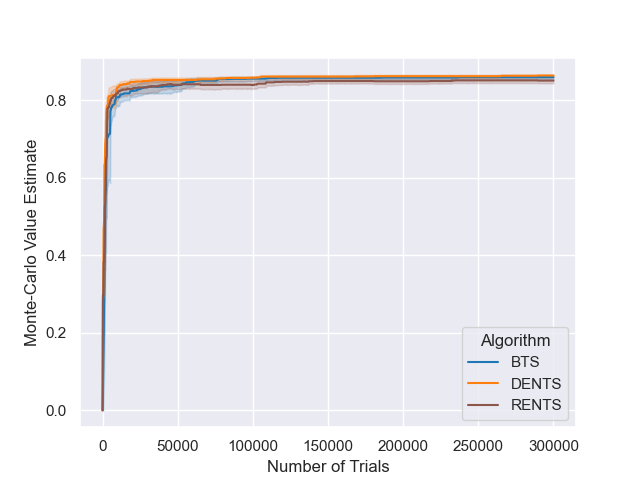
\includegraphics[width=\textwidth]{figures/temp/fl_sens/058_fl8_0_005_02.png}
                    \caption{$\alpha=0.005$}
                \end{subfigure}
                
                \caption{RENTS with a variety of temperatures on an 8x8 Frozen Lake environment. BTS and DENTS are included for reference. \todo{Update fig?}}
                \label{fig:fl_param_sens_rents}
            \end{figure}
            
            \begin{figure}
                \centering
                
                \begin{subfigure}[b]{0.32\textwidth}
                    \centering
                    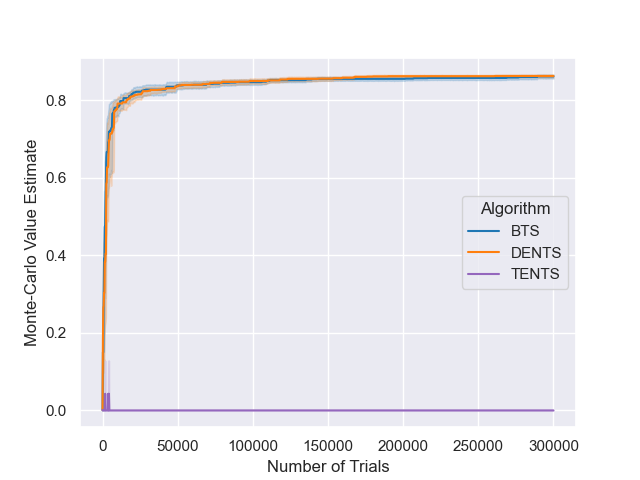
\includegraphics[width=\textwidth]{figures/temp/fl_sens/053_fl8_1_0_03.png}
                    \caption{$\alpha=1$}
                \end{subfigure}
                \begin{subfigure}[b]{0.32\textwidth}
                    \centering
                    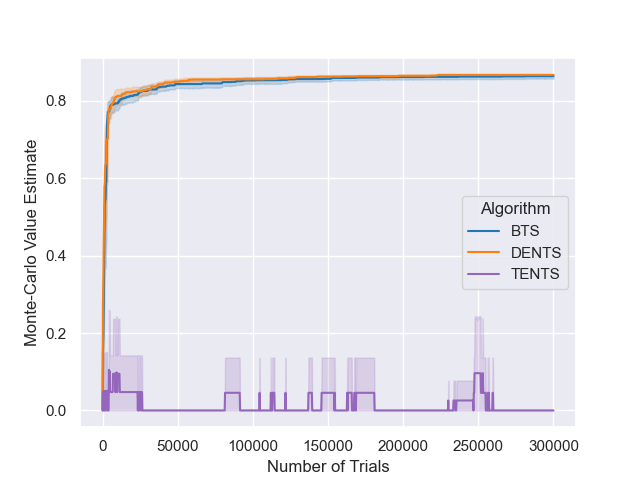
\includegraphics[width=\textwidth]{figures/temp/fl_sens/054_fl8_0_5_03.png}
                    \caption{$\alpha=0.5$}
                \end{subfigure}
                \begin{subfigure}[b]{0.32\textwidth}
                    \centering
                    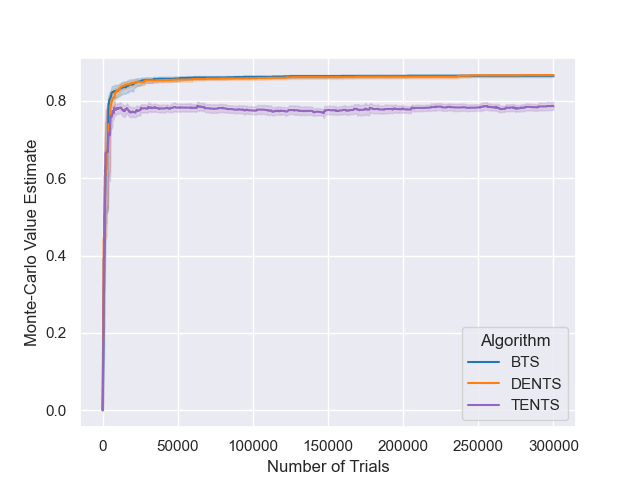
\includegraphics[width=\textwidth]{figures/temp/fl_sens/055_fl8_0_1_03.png}
                    \caption{$\alpha=0.1$}
                \end{subfigure}
                
                \begin{subfigure}[b]{0.32\textwidth}
                    \centering
                    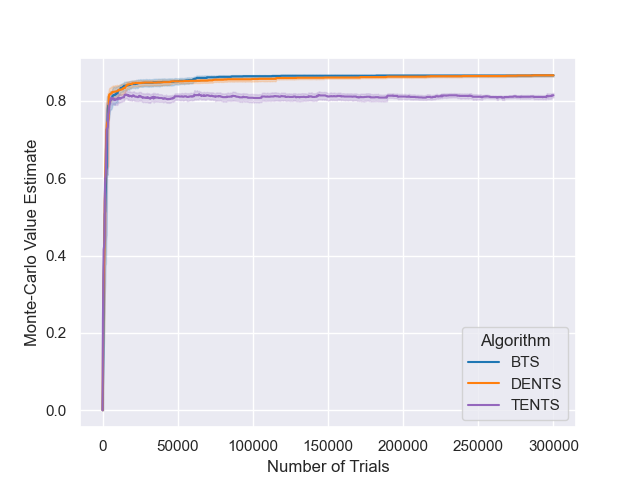
\includegraphics[width=\textwidth]{figures/temp/fl_sens/056_fl8_0_05_03.png}
                    \caption{$\alpha=0.05$}
                \end{subfigure}
                \begin{subfigure}[b]{0.32\textwidth}
                    \centering
                    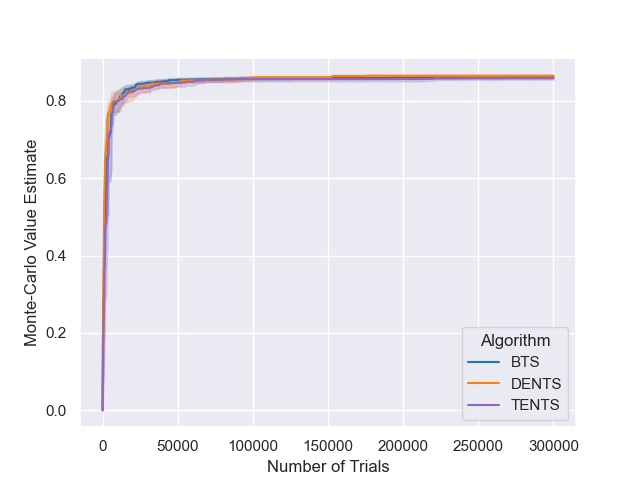
\includegraphics[width=\textwidth]{figures/temp/fl_sens/057_fl8_0_01_03.png}
                    \caption{$\alpha=0.01$}
                \end{subfigure}
                \begin{subfigure}[b]{0.32\textwidth}
                    \centering
                    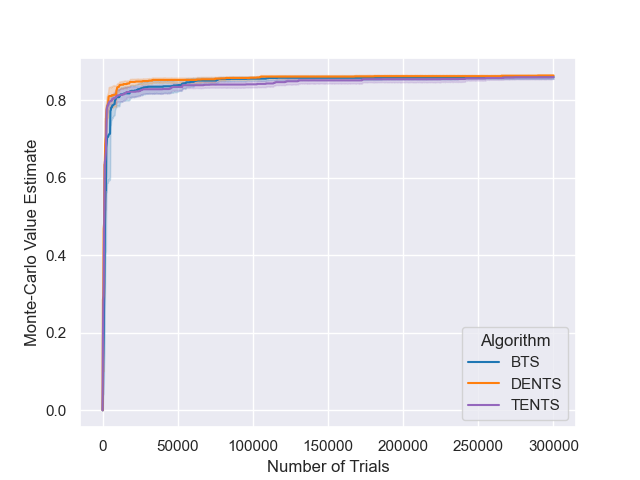
\includegraphics[width=\textwidth]{figures/temp/fl_sens/058_fl8_0_005_03.png}
                    \caption{$\alpha=0.005$}
                \end{subfigure}
                
                \caption{TENTS with a variety of temperatures on an 8x8 Frozen Lake environment. BTS and DENTS are included for reference. \todo{Update fig?}}
                \label{fig:fl_param_sens_tents}
            \end{figure}



        \subsubsection{Gridworld Results}

            \htodo{this subsubsection currently just a c and p from neurips}

            The 8x12 Frozen Lake environment (Figure \ref{fig:fl12}) and a 6x6 Sailing Problem (Figure \ref{fig:sailing_deets}) were used to evaluate the algorithms introduced in this chapter against the baseline algorithms.

            Each algorithm is run 25 times on each environment and evaluated every 250 trials using 250 trajectories. 
            A horizon of 100 was used for Frozen Lake and 50 for the Sailing Problem. Curves of these evaluations are given in Figure \ref{fig:gridworld_results}.

            In Frozen Lake (Figure \ref{fig:fl}), entropy proved to be a useful exploration bonus for the \textit{sparse reward}. Values in UCT and BTS remain at zero until a trial successfully reaches the goal. However, entropy guides agents to avoid trap states, where the entropy is zero. DENTS was able to perform similarly to MENTS, and BTS was able to improve its policy over time more than UCT.

            In the Sailing Problem (Figure \ref{fig:sp}) UCT performs well due to the dense reward. \htodo{also mention how exploiting is useful to get better value estimates in stochastic environments.} BTS and DENTS also manage to keep up with UCT. MENTS and TENTS appear to be slightly hindered by entropy in this environment. The relative entropy encourages RENTS to pick the same actions over time, so it tends to pick a direction and stick with it regardless of cost.
            
            Finally, BTS and DENTS were able to perform well in both domains with a sparse and dense reward structure, whereas the existing methods performed better on one than the other, hence making BTS and DENTS good candidates for a general purpose MCTS algorithm.

            \htodo{Say here that the initial wind directions for Sailing we set to North, and South-East.}
            
            \begin{figure*}
                \centering
                \begin{subfigure}[b]{0.49\textwidth}
                    \centering
                    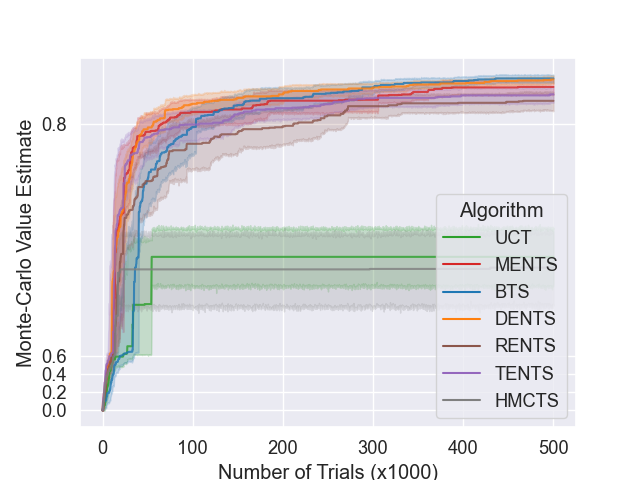
\includegraphics[width=\textwidth]{figures/temp/grid/fl.png}
                    \caption{8x12 Frozen Lake.}
                    \label{fig:fl}
                \end{subfigure}
                \begin{subfigure}[b]{0.49\textwidth}
                    \centering
                    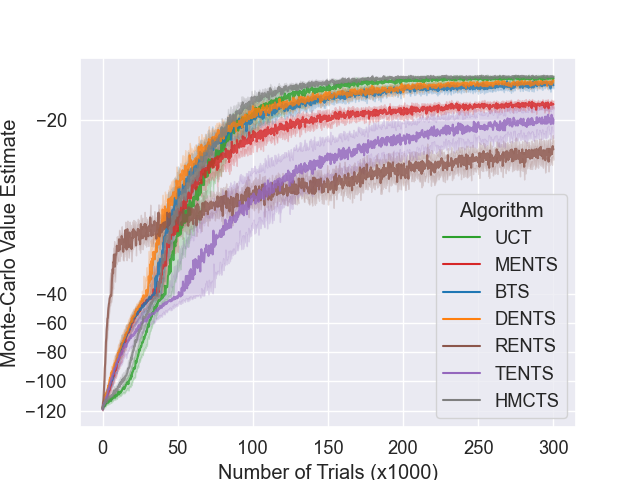
\includegraphics[width=\textwidth]{figures/temp/grid/s.png}
                    \caption{6x6 Sailing Problem.}
                    \label{fig:sp}
                \end{subfigure}
                \caption{Results for gridworld environments. \todo{update fig?} \htodo{add more caption?}}
                \label{fig:gridworld_results}
            \end{figure*}





        \subsubsection{Go Results}

            Results of the round-robin are summarised in Table \ref{table:go_results}, where each algorithm played $50$ games as black and $50$ as white. BTS was able to run the most trials per move and beat all of the other algorithms other than DENTS which it drew. The Alias method allowed the Boltzmann search algorithms to run significantly more trials per move than PUCT. BTS and DENTS were able to beat PUCT with results of 57-43 and 58-42 respectively. Using entropy did not seem to have much benefit in these experiments, as can be witnessed by MENTS only beating TENTS, and DENTS drawing 50-50 with BTS. This is likely because the additional exploration provided by entropy is vastly outweighed by utilising the information contained in the neural networks $\tilde{V}$ and $\tilde{\pi}$. Interestingly RENTS had the best performance out of the prior works, losing 43-57 to PUCT, and the use of relative entropy appears to take advantage of a heuristic for Go that the RAVE \cite{rave} algorithm used: the value of a move is typically unaffected by other moves on the board.
            
            To validate the strength of the \thtspp\ewe PUCT agent, it was played directly against KataGo \cite{katago}, with a budget of 1600~trials per move. Interestingly, the \thtspp\ewe PUCT agent won 61-39 in 9x9 Go, and lost 35-65 in 19x19 Go, suggesting that our PUCT agent is strong enough to provide a meaningful comparison for our other general purpose algorithms. Finally, note that the neural networks from KataGo were not fine-tuned, so the Boltzmann search algorithms directly used the networks that were trained for use in PUCT (with average returns).
            
          	

        \begin{table*}[]
        \centering   
		    \begin{tabular}{l|cccccc|c} 
		        \textbf{Black \textbackslash White}     & PUCT  & AR-M  & AR-R  & AR-T  & AR-B  & AR-D   & Trials/move\\ 
		        \hline
		                                PUCT            &   -   & 33-17 & 27-23 & 42-8  & 17-33 & 15-35  & 1054 \\
		                                AR-MENTS        & 12-48 &   -   & 13-37 & 38-12 & 10-40 & 12-38  & 4851\\
		                                AR-RENTS        & 20-30 & 24-26 &   -   & 39-11 & 18-32 & 14-36  & 3672 \\
		                                AR-TENTS        &  8-42 & 11-39 &  9-41 &   -   &  6-44 & 10-40  & 5206 \\
		                                AR-BTS          & 25-25 & 35-15 & 31-19 & 34-16 &   -   & 15-35  & 5375 \\
		                                AR-DENTS        & 23-27 & 36-14 & 29-21 & 36-14 & 15-35 &   -    & 4677 \\         
		    \end{tabular}
            \caption{Results for the Go round-robin tournament. The first column gives the agent playing as black. The final column gives the average trials run per move across the entire round-robin. In the top row, we abbreviate the algorithm names for space.\label{table:go_results}}
        \end{table*}



































        
            
            
            
            
            






























\section{Theoretical Results}
\label{sec:4-5-theory}

    \htodo{Change N(s,m) to N(s,n) and then change N(s,n) to N to pow n of s.}

    \htodo{Highlight where and when the actual theorems from the text come up. And make sure that they're clearly stated.}


    This Section provides the theoretical analysis and proofs discussed in this chapter. This section is structured as follows:
    \begin{enumerate}
        \item First, in Section \ref{sec:4-5-1-notation}, additional notation is defined so that the MCTS process can be reasoned about with respect to the number of trials run;
        \item Second, in Section \ref{sec:4-5-2-prelim}, \bd{some preliminary results, lemmas and definitions are given that are used in later results};
        \item Third, in Section \ref{sec:4-5-3-consistency}, the consistency results for (AR-)BTS and (AR-)DENTS are proven (Theorems \ref{thrm:4:bts}, \ref{thrm:4:bts_decay}, \ref{thrm:4:ar_bts}, \ref{thrm:4:dents}, \ref{thrm:4:dents_decay}, \ref{thrm:4:ar_dents}); 
        \item Fourth, in Section \ref{sec:4-5-4-entropy-trap}, Theorem \ref{thrm:ments_fail} is proven, showing that the maximum entropy objective is either misaligned or \bd{not useful} in the Entropy Trap problem from Section \ref{sec:4-3-toyenvs};
    \end{enumerate}

    Some of the particularly verbose arguments are left to Appendix \ref{app:theory-ch4} so that they do not distract from the string of thought in this section. In particular, Theorems \ref{thrm:4:bts_exp} and \ref{thrm:4:dents_exp}, which show exponential simple regret bounds on BTS and DENTS are left to Appendix \ref{appsec:exp}. This section will refer to particular parts of the appendix where they provide any relevant extra details. \htodo{also point the MENTS exp bound to this section, once that's written up}






\subsection{Notation}
\label{sec:4-5-1-notation}

    Firstly some additional notation is needed to be able to reason about the MCTS processes over time. Specifically, notation is needed to reason about random variables that vary with the number of MCTS trials run. Similarly to the main text, the assumption that for any two states $s,s'\in\cl{S}$ that $s=s'$ if and only if the trajectories leading to them are identical is made. This assumption is purely to simplify notation, so that nodes in the tree have a one-to-one correspondence with states (or state-action pairs). \todo{Either say because this assumption is made, can take an arbitrary} $s_t\in\cl{S}$ \todo{where t denotes the timestep where it can appear, because trajectories unique. OR, try to clean up that we sometimes use an arbitrary st from S. Its probably quite confusion.}

    When making arguments that apply to multiple algorithms the general policies $\pi$ and $\psi$ will be used, and when making arguments about specific algorithms the subscripts will be used, such as $\pibts$.

    Most variables be denoted with a superscript $n$ to denote that it is the value used on the $n$th trial of MCTS. For example:
    \begin{itemize}
        \item 
            If the algorithm uses a search policy $\pi$ and outputs a recommendation policy $\psi$, then the search policy followed on the $n$th trial is $\pi^n$, and the recommendation policy after $n$ trials is denoted $\psi^n$. 
        \item 
            When it is necessary to reason about multiple trajectories, the superscript notation will also be used. The trajectory sampled in the $n$th trial is $\tau^n=(s_0^n,a_0^n,r_0^n,...,s_{h-1}^n,a_{h-1}^n,r_{h-1}^n,s_{h}^n)$. If it is sampled from a search policy $\pi$, then $\tau^n\sim\pi^n$.
        \item 
            The search tree after $n$ trials is denoted $\cl{T}^n$, the initial search tree is $\cl{T}^0=\{s_0\}$, and $\cl{T}^n = \cl{T}^{n-1} \cup \tau^n$.
    \end{itemize}

    It will also be useful to have some additional notation for counting the number of times that nodes have been visited. Let the $m$th trajectory be $\tau^m=(s_0^m,a_0^m,r_0^m,...,s_{h-1}^m,a_{h-1}^m,r_{h-1}^m,s_{h}^m)$ for $1\leq m \leq n$. The number of times state~$s_t$ was visited in the first $n$ trials is $N^n(s_t)$, and the number of times action~$a_t$ was selected from state~$s_t$ in the first $n$ trials is $N^n(s_t,a_t)$. \htodo{make rest of text consistent with this notation.} Also, let $T^n(s_t)$ (and $T^n(s_t,a_t)$) be the set of trajectory indices that $s_t$ was visited on (and action $a_t$ selected) in the first $n$ trials: 
    %
    \begin{align}
        T^n(s_t) &= \{i | 1\leq i\leq n, s^i_t = s_t \} \\
        T^n(s_t,a_t) &= \{i | 1\leq i\leq n, s^i_t = s_t, a^i_t = a_t \}.
    \end{align}
    %
    This allows the counts $N^n(s_t),$ $N^n(s_t,a_t)$ and $N^n(s_{t+1})$ (with $s_{t+1}\in\suc{s_t}{a_t}$) to be written as sums of indicator random variables in the following ways:
    %
    \begin{align}
        N^n(s_t) &= \sum_{i=1}^n \one[s^i_t=s_t] = |T(s_t,m)|, \\
        N^n(s_t,a_t) &= \sum_{i=1}^n \one[s^i_t=s_t,a^i_t=a_t] = |T(s_t,a_t,m)|, \\ 
        N^n(s_t,a_t) &= \sum_{i\in T^n(s_t)} \one[a^i_t = a_t], \label{appeq:nsa_sum} \\
        N^n(s_{t+1}) &= \sum_{i\in T^n(s_t,a_t)} \one[s^i_{t+1} = s_{t+1}]. \label{appeq:ns_sum}
    \end{align}
    %

    The exception to the superscript notation with respect to the number of trials will be value estimates. They will instead be denoted with respect to the number of times the value has been backed up. To clearly differentiate this counting with respect to backups, instead of with respect to trials, a superscript with brackets will be used. For example, the backups for DENTS value estimates would be written as follows. Let $\tau^n \sim \mpidents{n}$ and $\tau^n=(s_0,a_0,r_0,...,s_{h-1},a_{h-1},r_{h-1},s_{h})$, the backups for $t=h-1,...,0$ are: 
    %
    \begin{align}
        \mQdents{N^n(s_t,a_t)}(s_t,a_t) &= 
            R(s_t,a_t) + \sum_{s' \in \suc{s_t}{a_t}} \left( 
                \frac{N^n(s')}{N^n(s_t,a_t)} \mVdents{N^n(s')}(s') \right), 
            \label{appeq:dp_q_backup} \\ 
        \mVdents{N^n(s_t)}(s_t) &=\max_{a\in\cl{A}} \mQdents{N^n(s_t,a)}(s_t,a), 
            \label{appeq:dp_v_backup} \\
        \mHQdents{N^n(s_t,a_t)}(s_t,a_t) &= 
            \sum_{s'\in \suc{s_t}{a_t}} \frac{N^n(s')}{N^n(s_t,a_t)} \mHVdents{N^n(s')}(s'), \\
        \mHVdents{N^n(s_t)}(s_t) &= 
            \cl{H}(\mpidents{n}(\cdot | s_t)) 
                + \sum_{a\in\cl{A}} \mpidents{n}(a_t|s_t)\mHQdents{N^n(s_t,a_t)}(s_t,a_t).
    \end{align}
    %
    \todo{Double check we've actually defined the value at leaf nodes as Vinit somewhere in the thesis at least. And make a comment about it here?}
    
    For reference, all of the algorithms considered in this Section are written out in full with this additional notation in Appendix \ref{appsec:mcts_stoch_process}.















    \subsection{Preliminaries}
    \label{sec:4-5-2-prelim}

        Firstly, it is worth noting that mathematically (AR-)BTS is a special case of (AR-)DENTS, with $\betadents(x)=0$ and $\betaardents(x)=0$. Results will be proven about (AR-)DENTS, and the corresponding results for BTS follow from setting the entropy weighting function to zero.





        \begin{defn}
            A sequence of random variables $X_i$ \textnormal{converges in probability} to a random variable $X$, written as $X_n \rap X$, if for all $\varepsilon>0$ the following holds:
            \begin{align}
                \Pr\left(\left|X_n - X\right| > \varepsilon\right) \rightarrow 0 \ \text{as} \ n \rightarrow \infty.
            \end{align}
        \end{defn}

        \begin{defn}
            A sequence of random variables $X_i$ \textnormal{converges almost surely} to a random variable $X$, written as $X_n \raas X$, if the following holds:
            \begin{align}
                \Pr\left(\lim_{n\rightarrow\infty} X_n = X\right) = 1.
            \end{align}
        \end{defn}
        




        % \todo{DEFINITELY APPENDIX MATERIAL}

        % This section revisits \textit{simple regret} in more detail. Recall the definition of simple regret \todo{double check this is correct notation (brain ded today)}:
        % %
        % \begin{align} 
        %     \sreg(s_t,\psi^n) &= V^*(s_t) - V^{\psi^n}(s_t), 
        % \end{align}
        % %
        % where $\psi^n$ is the policy recommended after $n$ rounds or trials. 
        
        The definition of simple regret (Definition \ref{def:2:simple_regret}) used in this thesis is different to what has been considered by the tree search literature so far \todo{cite: mcts\_simple\_regret,brue1}, which only considers the \textit{immediate regret} of taking a single action step. However, the definition used in this thesis is a more natural extension to the simple regret considered for multi-armed bandit problems \todo{cite: simple\_regret\_short,simple\_regret\_long}, as it stems from a more general MDP planning problem that does not have to be solved using a tree search. For example, consider a non-tree search algorithm that outputs a recommendation policy rather than one action at a time. 

        However, the \textit{immediate simple regret} will be a simpler quantity to work with for proofs:
        \begin{defn}
            The \textnormal{immediate simple regret} is defined as as:
            %
            \begin{align}
                \immreg_I(s_t,\psi^n) =& V^*(s) - \bb{E}_{a_t\sim\psi^n(s_t)}[Q^*(s_t,a_t)].
            \end{align}
        \end{defn}

        The differences between these alternative definitions of simple regret can be reconciled by showing that any bound and convergence results that hold for one must also hold for the other.

        \begin{lemma} \label{lem:imm_simple_regret}
            $\bb{E}\sreg(s_t,\psi^n)=O(f(n))$ for all $s_t\in\cl{S}$ iff $\bb{E}\immreg(s_t,\psi^n)=O(f(n))$ for all $s_t\in\cl{S}$. Consequently, $\bb{E}\sreg(s_t,\psi^n)\rightarrow 0$ iff $\bb{E}\immreg(s_t,\psi^n)\rightarrow 0$.
        \end{lemma}
        \begin{proof}
            Firstly, notice that the simple regret can be written recursively in terms of the immediate simple regret:
            \begin{align}
                \sreg(s_t,\psi^n) =& V^*(s_t) - V^{\psi^n}(s_t) \\
                    =& V^*(s_t) - \bb{E}_{a_t\sim\psi^n(s)}[Q^{\psi^n}(s_t,a_t)] \\
                    =& V^*(s_t) - \bb{E}_{a_t\sim\psi^n(s)}[R(s_t,a_t) +    
                        \bb{E}_{s_{t+1}\sim\Pr(\cdot|s_t,a_t)}[V^{\psi^n}(s_{t+1})]] \\
                    =& V^*(s_t) - \bb{E}_{a_t\sim\psi^n(s)}\big[Q^*(s,a) - 
                        \bb{E}_{s_{t+1}\sim\Pr(\cdot|s_t,a_t)}[V^*(s_{t+1})]  \notag \\
                        &+ \bb{E}_{s_{t+1}\sim\Pr(\cdot|s_t,a_t)}[V^{\psi^n}(s_{t+1})]\big] \label{eq:simple_reg} \\
                    =& V^*(s_t) - \bb{E}_{a_t\sim\psi^n(s_t)}[Q^*(s_t,a_t)] \notag \\
                        &+ \bb{E}_{a_t\sim\psi_n(s_t),s_{t+1}\sim\Pr(\cdot|s_t,a_t)}[
                            V^*(s_{t+1}) - V^{\psi^n}(s_{t+1})] \\
                    =& \immreg(s,\psi^n) + 
                        \bb{E}_{a_t\sim\psi^n(s_t),s'\sim\Pr(\cdot|s_t,a_t)}[\sreg(s_{t+1},\psi^n)], \label{eq:regret_relation}
            \end{align}
            where line (\ref{eq:simple_reg}) uses $R(s,a) = Q^*(s,a) - \bb{E}_{s'\sim\Pr(\cdot|s,a)}[V^*(s')]$, a rearrangement of the Bellman optimality equation for $Q^*(s,a)$.
            
            This shows that if $\bb{E}\sreg(s_t,\psi^n)=O(f(n))$ then $\bb{E}\immreg(s_t,\psi^n)\leq \bb{E}\sreg(s_t,\psi^n) = O(f(n))$. Now suppose that $\bb{E}\immreg(s_t,\psi^n)=O(f(n))$ and assume an inductive hypothesis that $\bb{E}\sreg(s_{t+1},\psi^n)=O(f(n))$ for all $s_{t+1}\in\bigcup_{a\in\cl{A}}\suc{s_t}{a}$, then:
            \begin{align}
                \bb{E}\sreg(s_t,\psi^n) = \bb{E}\left[ O(f(n)) + \bb{E}_{a_t\sim\psi^n(s_t),s_{t+1}\sim\Pr(\cdot|s_t,a_t)}[O(f(n))] \right] = O(f(n)),
            \end{align}
            where the outer expectation is with respect $\psi^n$ (as the recommendation policy is the output of a random process).

            \todo{Setting f(n) equal to one of the expected simple regret gives the last bit. As f(n) is O(f(n)).}
        \end{proof}





        \htodo{Commented out corollary below. As we're now making N(s,a,n) explicit, exp(-kN(s,a,n)) is an f(n), so the above lemma is sufficient to handle the below.}
        
        \htodo{Change any references to cor:imm\_to\_full\_simple\_regret to lem:imm\_simple\_regret instead.}

        % It is useful to specialise Lemma \ref{lem:imm_simple_regret} specifically for the form of bounds used later. I.e. the simple regret at $s_t$ admits a regret bound exponential in $N(s_t)$, if and only if, the immediate simple regret admits a bound exponential in $N(s_t)$.
        
        % \begin{corollary} \label{cor:imm_to_full_simple_regret}
        %     Consider any Boltzmann MCTS process. There exists $C_1,k_1>0$ such that $\bb{E}\sreg(s_t,\psi^n) \leq C_1\exp(-k_1 N(s_t))$ iff there exists $C_2,k_2>0$ such that $\bb{E}\immreg(s_t,\psi^n) \leq C_2\exp(-k_2 N(s_t))$.
        % \end{corollary}
        % \begin{proofoutline}
        %     The proof follows similarly to Lemma \ref{lem:imm_simple_regret}. The additional nuance is that we need to apply Lemmas \ref{lem:sa_to_s} and \ref{lem:s_to_sa}. Note that the assumption of a minimum action probability in Lemma \ref{lem:sa_to_s} is satisfied, because there is a minimum positive probability of selecting an action in any Boltzmann MCTS process (Lemma \ref{lem:min_prob}). The inductive hypothesis for $s_{t+1}\in\bigcup_{a\in\cl{A}}\suc{s_t}{a}$ would give a bound with respect to $N(s_{t+1})$, and the lemmas are required to `translate' the bound into one with respect to $N(s_t)$.
        % \end{proofoutline}
            
            






















    \subsection{Consistency Results} 
    \label{sec:4-5-3-consistency}

        \bd{This subsection gives consistency results for (AR-)DENTS and consequently (AR-)BTS. It begins by showing that the Boltzmann search policies will lead to every state and state-action pair being visited infinitely often. Then a lot of inductive step lemmas, and then finally its all tied up in the theorems using inductive arguments.}









        \todo{All nodes visited infinitely often}









        \todo{Make this the main section showing consistency of Boltzmann MCTS processes and under what conditions. Have the missing proofs written up on ipad.}
    
        \todo{Also write up the general steps from the ipad notes (which I think need a bit of correction.)}
    
        Because the search temperature is now decayed, \todo{we} need to show that the exploration term in the search policies leads to actions being sampled infinitely often.
    
    
        \todo{This lemma restated means that Boltzmann search policies will select all actions infinitely often.}
        \todo{Check the variables in this proof are consistent with the definitions of N(s,a,m) etc}
    
        \begin{lemma} \label{lem:inf_often_action_select}
            Let $\rho^m$ be an arbitrary policy, and the following policy: \todo{handle when epsilon is greater than one? I think its just let ell be large enough argument}
            \begin{align} 
                \pi^m(a)=(1-\lambda(m))\rho^m(a) + \lambda(m) \frac{1}{|\cl{A}|}, \label{appeq:ioas_policy}
            \end{align} 
            with $\lambda(m)=\min(1,\epsilon/\log(e+m))$, where $\epsilon\in(0,\infty)$. Let $a^m\sim \pi^m$ be the $m$th sampled action, and let $M(a,m)$ be the number of times action $a$ was selected in the first $m$ samples, i.e. $M(a,m)=\sum_{m=1}^m \one[a^m=a]$. Then for all $a\in\cl{A}$ we have $M(a,m)\raas\infty$ as $m\rightarrow \infty$.
        \end{lemma}
        \begin{proof}
            First consider that if $M(a,m)\not\rightarrow\infty$ then it is logically equivalent to say that there exists some $\ell$ such that from $a^\ell$ onwards that there is some action which is never sampled again. To prove the result, argue by contradiction, and suppose that there is some $\ell\in\bb{N}$ and $b\in\cl{A}$ such that:
            \begin{align}
                \Pr\left(\bigcap_{m=\ell}^\infty a^m \neq b\right) > 0. \label{appeq:ioas_contradict}
            \end{align}
    
            However, from the definition of equation (\ref{appeq:ioas_policy}) it must be that:
            \begin{align}
                \Pr\left(a^m = b\right) \geq \frac{\lambda(m)}{|\cl{A}|} = \frac{\epsilon}{|\cl{A}| \log(e+m)}.
            \end{align} 
    
            And so using this lower bound to work out the probability of never sampling action $b$ again after the first $\ell-1$ samples gives:
            \begin{align}
                \Pr\left(\bigcap_{m=\ell}^\infty a^m \neq b \right)
                    &= \lim_{k\rightarrow\infty} \prod_{m=\ell}^k 
                        \Pr(a^m \neq b) \\
                    &\leq \lim_{k\rightarrow\infty} \prod_{m=\ell}^k 
                        \left( 1 - \frac{\epsilon}{|\cl{A}|\log(e+k)} \right) \\
                    &\leq \lim_{k\rightarrow\infty} 
                        \left( 1 - \frac{\epsilon}{|\cl{A}|\log(e+k)} \right)^{k-\ell} \label{appeq:ioas_one} \\
                    &= 0, \label{appeq:ioas_two}
            \end{align}
            %
            which is in contradiction to inequality (\ref{appeq:ioas_contradict}) that was assumed. Inequality (\ref{appeq:ioas_one}) holds because the factors in the product are increasing with respect to $m$. To see why the final limit equality (\ref{appeq:ioas_two}) holds, consider the simpler function $f(x)=\left(1-1/\log(x)\right)^x$. Taking logarithms and applying L'Hopital's rule \todo{cite?} generously gives:
            \begin{align}
                \lim_{x\rightarrow \infty} \log f(x) 
                &= \lim_{x\rightarrow \infty} x \log\left(1-\frac{1}{\log(x)}\right) \\
                &= \lim_{x\rightarrow \infty} \frac{\log\left(1-\frac{1}{\log(x)}\right)}{x^{-1}} \\
                &= \lim_{x\rightarrow \infty} \frac{\frac{1}{x\log(x)(\log(x)-1)}}{-x^{-2}} \\
                &= \lim_{x\rightarrow \infty} \frac{-x}{\log(x)(\log(x)-1)} \\
                &= \lim_{x\rightarrow \infty} \frac{-x}{2\log(x)-1} \\
                &= \lim_{x\rightarrow \infty} \frac{-x}{2} \\
                &= -\infty.
            \end{align} 
            %
            And thus $\lim_{x\rightarrow\infty} f(x) = \lim_{y\rightarrow -\infty} e^{y} = 0$.
    
            \todo{cut this down maybe, its a little excessive showing all of the working out?}
    
            Hence, by contradiction, it must be the case that $\Pr(M(a,m)\not\rightarrow\infty) = 0$, or rather that $\Pr(M(a,m)\rightarrow\infty) = 1$ which is the desired result.
        \end{proof}
        %
        \todo{Can we also say that if its (1 - 1/o(x)) to the x, then it will generally hold, so x to the power of 0.99 could equally be used. And also any polynomial of log(x) could be used} 
    
        
    
    
    
    
    
    
        \todo{Words about the consequences of this lemma?}
    
        In direct consequence of Lemma \ref{lem:inf_often_action_select}, every reachable state (and state-action pair) will be visited infinitely often in a Boltzmann MCTS Process.
    
        \begin{corollary} \label{cor:inf_often_visit_node}
            For any Boltzmann MCTS Process (i.e. a MCTS algorithm using a search policy of the form $\pi^m(a)=(1-\lambda(m))\rho^m(a) + \lambda(m) \frac{1}{|\cl{A}|}$), all reachable states from the root node are visited infinitely often. Specifically, for any reachable $s\in\cl{S}$ is must be that $N(s,m)\raas\infty$ and $N(s,a,m)\raas\infty$ as $m\rightarrow\infty$. \todo{handle reachability somewhere better? just make some assumption at the start of the theory section saying we assume all s are reacahable?}
        \end{corollary}
        \begin{proofoutline}
            This is a direct consequence of Lemma \ref{lem:inf_often_action_select} when applied inductively at each node.
        \end{proofoutline}












        \todo{Now already get core BTS and DENTS results.} 

        \todo{DP backups converge in limit (Dynamic Programming cite)}

        \todo{And corollary is that DENTS with DP backups converges}

        Theorem \ref{thrm:4:dents} and \ref{thrm:4:bts}.

















        \todo{If Q values converge then can make search policy converge. Generalise the below to be for AR-DENTS and DENTS in one}





        \todo{Words about the below, which gives conditions for the search policy to tend to the optimal policy, and should add somewhere that can't have the search policy converge to the optimal policy and get exp simple regret convergence in theory}

        \begin{lemma}
            \todo{Write this up properly, and more generally, and use the indexed on num trials notation. Say that as long as the Q function converges to the optimal, beta is o(alpha) and alpha tends to zero, then search policy tends to optimal policy.}
            If $\Qardents(s,a)\rap Q^*(s,a)$ then $\piardents \rap \pi^*$
        \end{lemma}
    
        \begin{proofoutline}
            A full proof to show that these limits converge correctly needs to make use of the dominated convergence theorem \todo{cite}. Also use this argument hashed out with gpt https://chatgpt.com/c/67b632f2-0554-8007-9d6c-d24b10a3cf99
    
            The outline argument is that in $\piardents$ that firstly $\lambda \rightarrow 0$ and so the limit of $\piardents$ will be the same as the limit of $\rhoardents$. 
            
            \todo{Words about the below maths, and below is very informal writing up}
            \begin{align}
                \frac{1}{\alpha(n)}\dot{Q}(s,a) + \frac{\beta(n)}{\alpha(n)} \bar{\cl{H}}_Q(s,a) 
                    &\rightarrow \frac{1}{\alpha(n)}\dot{Q}(s,a) \\
                \rho(a|s) &\rightarrow \frac{1}{Z} \exp\left(\frac{\dot{Q}(s,a)}{\alpha(n)}\right) \\
                    &\rightarrow \one[a=a^*]
            \end{align}
    
            \todo{Should probably show that softmax converges to max in limit}
        \end{proofoutline}
















        \todo{if search policy converges, then most visited recommendation converge}


        \todo{Another proof about visits. For most visit recommendations, use this to justify that alpha can be arbitrary, but need beta equal to o(alpha), (which is alpha doesnt go to zero just means that beta goes to zero) in the DP case, and for the AR case need the same conditions with alpha to zero}
        \begin{lemma}
            \todo{write this up properly}
            If $\pi\rap\pi_{\lim}$ such that $\pi_{\lim}(a*|s)>\pi(a|s)$ for all $a,s$, then the most visited recommendation policy will converge. Specifically, $\frac{N(s,a,n)}{N(s,n)} \rap \pi_{\lim}(a|s)$.
        \end{lemma}
        \begin{proof}
            \todo{write this up properly}
            First use Kolmogorovs strong law \todo{cite the source downloaded}, which valid because $\sum\frac{\bb{E}\one[a^i=a]^2}{k^2} \leq \sum \frac{1}{k^2} < \infty$. Using this gives
            \begin{align}
                \frac{N(s,a,n)}{N(s,n)}
                    &= \frac{1}{N(s,n)} \sum_{i=1}^N(s,n) \one[a^i = a] \\
                    &\rightarrow \bb{E} \lim_{n\rightarrow\infty} \sum_{i=1}^n \frac{\one[a^i=a]}{n} \\
                    &= \lim_{n\rightarrow\infty} \bb{E} \sum_{i=1}^n \frac{\one[a^i=a]}{n} \\
                    &= \lim_{n\rightarrow\infty} \sum_{i=1}^n \frac{\pi^i(a|s)}{n} \\
                    &= \pi^i(a|s)
            \end{align}
    
            Where the last line uses if $x_n \rightarrow x$ then $\sum_{i=1}^n \frac{x_i}{n} \rightarrow x$. \todo{cite this somehow? Cesaro summation?}
        \end{proof}
    
        \todo{Write up results that use the above lemma to have consequence that most visited recommendation policy is consistent.}











        \todo{if search policy converges and Q values converge, then V values converge.}


        \todo{AR-DENTS can use the generalised Q convergence result, via the equations above still.}

        \todo{AR-DENTS needs three steps for the induction, with the extra step of if Q values converge then policy converges as given above}

        \begin{lemma}
            \todo{clean up this writing}
            If $\piardents\rap\pi^*$ (i.e. \todo{conditions from above result}), and $\Qardents \rap Q^*$, then $\Vardents \rap V^*$.
        \end{lemma}
        \begin{proofoutline}
            \todo{clean}
            Using the result above \todo{ref}, it must be that $\piardents(a|s) \rightarrow \pi^*(a|s) = \one[a^*_{|s} = a]$. Then recalling equation \todo{ref} that related the average returns values:
            \begin{align}
                \bar{V}(s) &= \sum_{a} \frac{N(s,a,n)}{N(s,n)} \bar{Q}(s,a) \\
                    &\rap \sum_{a} \one[a^*_{|s}=a] \bar{Q}(s,a) \\
                    &= \bar{Q}(s,a^*_{|s}) \\
                    &\rap Q^*(s,a^*_{|s}) \\
                    &= V^*(s).
            \end{align}
        \end{proofoutline}









        \todo{Words about how doing the if V converges, the Q converges step.}

        

        \begin{theorem} \label{thrm:dkw_inequality}
            Let $\{X_i\}_{i=1}^m$ be random variables drawn from a probability distribution with a cumulative distribution function of $F$. Let the empirical cumulative distribution function be $F_m(x)=\frac{1}{m} \sum_{i=1}^m \one[X_i < x]$. Then the Dvoretzky-Kiefer-Wolfowitz inequality is:
            \begin{align}
                \Pr\left(\sup_x |F_m(x)-F(x)| > \varepsilon\right) \leq 2\exp\left(-2m\varepsilon^2\right).
            \end{align}
        \end{theorem}
        \begin{proof}
            See \todo{fix cite}%\citeapp{dvoretzky1956asymptotic}.
        \end{proof}
        

        The Dvoretzky-Kiefer-Wolfowitz inequality is of interest because it allows the empirical transition probability $N(s_{t+1},n)/N(s_t,a_t,n)$ to be tightly bounded with the true transition probability $p(s_{t+1}|s_t,a_t)$. 
        %
        \begin{figure}
            \centering
            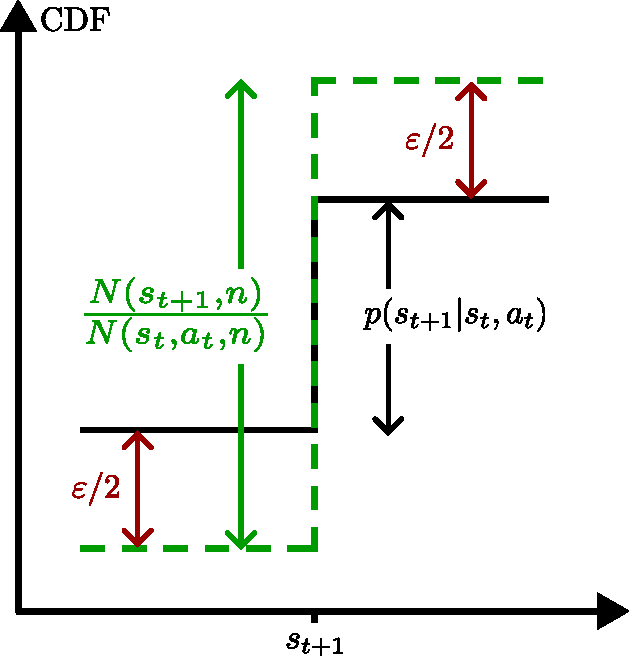
\includegraphics[scale=0.6]{figures/ch4/dkw_diagram.pdf}
            \caption[Bounding the empirical transition probabilities to the true transition probabilities.]{Bounding the empirical transition probabilities to the true transition probabilities. The true cdf is shown as a solid black line, the empirical cdf is shown as a dashed green line, and a worst case error of $\varepsilon/2$, using Theorem \ref{thrm:dkw_inequality}, is shown in red. The probability mass of $p(s_{t+1}|s_t,a_t)$ and empirical probability mass of $\frac{N(s_{t+1},n)}{N(s_t,a_t,n)}$ is also indicated to demonstrate how the constructed distribution gives Corollary \ref{cor:bound_transition_distribution}.}
            \label{fig:dkw_diag}
        \end{figure}
        %
        \begin{corollary} \label{cor:bound_transition_distribution}
            Consider any Boltzmann MCTS process. For all $(s_t,a_t)\in\cl{S}\times\cl{A}$ and for all $\varepsilon >0$ we have:
            \begin{align}
                \Pr\left(\max_{s_{t+1}\in\suc{s_t}{a_t}}\left| \frac{N(s_{t+1},n)}{N(s_t,a_t,n)} - p(s_{t+1}|s_t,a_t) \right| > \varepsilon \right) \leq 2 \exp\left(-\frac{1}{2}\varepsilon^2 N(s_t,a_t) \right).
            \end{align}
            %
            Consequently $\frac{N^n(s_{t+1})}{N^n(s_t,a_t)} \rap p(s_{t+1}|s_t,a_t)$.
        \end{corollary}
        \begin{proofoutline}
            By considering some arbitrary ordering over the successor states in $\suc{s_t}{a_t}$ and applying Theorem \ref{thrm:dkw_inequality}, replacing $\varepsilon$ by $\varepsilon/2$, the result follows.

            To see why the factor of $1/2$ is needed, consider Figure \ref{fig:dkw_diag}. Because the distribution is discrete, the cumulative distribution function is a (piecewise constant) step function. As Theorem \ref{thrm:dkw_inequality} bounds the maximum difference between the empirical and true cumulative distribution functions, the factor of $1/2$ is needed to account for the error before and after each $s_{t+1}$ in the worst case.

            \todo{Final bit holds by taking the limit, specify that it is with respect to N(s,a) tending to inf, not n this time. (Need to also use that N(s,a) goes to inf as n goes to inf from above)}
        \end{proofoutline}


        \todo{Result of how if V rap V*, then Q rap Q*. Follows immediately from the corollary above.}













        \todo{Give the final theorems} Theorems \ref{thrm:4:bts_decay}, \ref{thrm:4:ar_bts}, \ref{thrm:4:dents_decay}, \ref{thrm:4:ar_dents}
  











        \todo{Use customthrms, repeat the BTS theorems, and say that they hold from setting beta to zero in the DENTS theorems above.}
    
        % \begin{customthm}{4.1}
        %     For any MDP $\cl{M}$, after running $n$ trials of the BTS algorithm with a root node of $s_0$, there exists constants $C,k>0$ such that for all $\varepsilon>0$ we have $\bb{E}[\reg(s_0,\psi^n_{\textnormal{BTS}})] \leq C\exp(-kn)$, and also $\Vt{s_0}{N(s_0)} \rap V^*(s_0)$ as $n\rightarrow\infty$.
        % \end{customthm}
        % \begin{proof}
        %     Follows from setting $\beta(m)=0$ and using Theorem \ref{thrm:dents}.
        % \end{proof}




















        \todo{This was before the AR proofs originally. Should really just make sure that this is covered in the UCT section in Ch2, and then recall it. Either in the preliminaries, or before the first place its needed in this chapter here where roughly here where it's needed.}

        \todo{SOME of this should be integrated into the main arguments I think}

        \todo{N(s) to N(s,n) stuff}

        In this section informal proof outlines for theoretical results for AR-BTS and AR-DENTS are given. To begin with define the average return $\bar{V}^{N(s)}(s)$ for a decision node at $s$, and recall the definition of $\bar{Q}^{N(s,a)}(s, a)$:

        \begin{align}
            \bar{V}^{N(s_t)+1}(s_t) &= \bar{V}^{N(s_t)}(s_t) + \frac{\bar{R}(s_t) - \bar{V}^{N(s_t)}(s_t)}{N(s_t) + 1},  \label{appeq:ar_v} \\
            \bar{Q}^{N(s_t,a_t)+1}(s_t, a_t) &= \bar{Q}^{N(s_t,a_t)}(s_t, a_t) 
                + \frac{\bar{R}(s_t,a_t) - \bar{Q}^{N(s_t,a_t)}(s_t, a_t)}{N(s_t, a_t) + 1},  \label{appeq:ar_q}
        \end{align}
        %
        where $\bar{R}(s_t)=\sum_{i=t}^H R(s_i,a_i)$ and $\bar{R}(s_t, a_t)=\sum_{i=t}^H R(s_i,a_i)$. Note that these average return values also satisfy the equations:
        %
        \begin{align}
            \bar{V}^{N(s_t)}(s_t) &= \sum_{a\in\cl{A}} \frac{N(s_t,a)}{N(s_t)} \bar{Q}^{N(s_t,a_t)}(s_t, a_t), \label{appeq:ar_v_rel} \\
            \bar{Q}^{N(s_t,a_t)}(s_t, a_t) 
                &= R(s_t,a_t) + \sum_{a\in\cl{A}} \frac{N(s')}{N(s_t,a_t)} \bar{V}^{N(s')}(s'). \label{appeq:ar_q_rel}
        \end{align}
        %
        \todo{should we do the rearrangement/working out for this?}











        \todo{Necessity for ar-bts to have temp tend to zero, but would need to change the theorem to say lower bound on temp rather than just fixed temp.}
        Firstly, it can be shown that using a non-decaying search temperature with AR-BTS is not guaranteed to recommend the optimal policy.
        
        \begin{figure}
            \centering
            
\includegraphics[width=0.7\textwidth]{figures/todo.jpg}
            \caption{\todo{Haven't touched this, need to reproduce from neurips paper}An MDP that AR-BTS will not converge to recommending the optimal policy on, for a large enough value of $D$.}
            \label{fig:ar_gen_mdp}
        \end{figure}

        \begin{customprop}{B.1}
            \todo{Haven't touched this, just c and p from neurips paper}

            For any $\alpha_{\textnormal{fix}}>0$, there is an MDP $\cl{M}$ such that AR-BTS with $\alpha(m)=\alpha_{\textnormal{fix}}$ is not consistent: $\bb{E}[\sreg(s_0,\psi^n_{\textnormal{AR-BTS}})] \not\to 0$ as $n\to\infty$. 
        \end{customprop}
        \begin{proofoutline}
            \todo{Haven't touched this, just c and p from neurips paper}

            Consider the MDP given in Figure \ref{fig:ar_gen_mdp}. We can show inductively that (as $n\rightarrow\infty$) the value of $\bb{E}\bar{V}^{N(k)}(k)\leq 2E^{D-k+1} < 2$, where $E=e^2/(1+e^2)$ for $2\leq k \leq D$. The inductive step is as follows:
            \begin{align}
                \bb{E}\bar{V}^{N(k)}(k) =& \frac{\exp\left(\bar{V}^{N(k+1)}(k+1)\right)}{1+\exp\left(\bar{V}^{N(k+1)}(k+1)\right)} \bb{E}\bar{V}^{N(k+1)}(k+1) 
                    + \frac{1}{1+\exp\left(\bar{V}^{N(k+1)}(k+1)\right)} \cdot 0 \\
                    \leq& E \cdot \bb{E} \bar{V}^{N(k+1)}(k+1) \\
                    \leq& E \cdot 2E^{D-k} \\
                    =& 2E^{D-k+1}.
            \end{align}

            where we know that $\exp\left(\bar{V}^{N(k+1)}(k+1)\right)/\left(1+\exp\left(\bar{V}^{N(k+1)}(k+1)\right)\right) < E$, because the function $e^x/(1+e^x)$ is monotonically increasing in $x$, and $\bar{V}^{N(k+1)}(k+1) < 2$. Hence, by choosing an integer $D$ such that $D-1 \geq \log(1/3) / \log(E)$, we have $\bb{E}\bar{V}^{N(2)}(2)=2E^{D-1}\leq 2/3 < 1 = \bb{E}\bar{Q}^{N(1,a_2)}(1,a_2)$. 

            A full proof should show that AR-BTS does indeed converge to these expected values, possibly through concentration bounds. 
            \todo{(was camera ready todo) Do the full proof, and show that AR-BTS converges to these value with non zero prob, hence the non zero simple regret.} 

            Hence, AR-BTS does not converge to a simple regret of zero, because the expected Q-values as $n\rightarrow\infty$ are $\bb{E}\bar{Q}^{N(1,a_2)}(1,a_2)=1$ and $\bb{E}\bar{Q}^{N(1,a_1)}(1,a_1)<2/3$, so AR-BTS would incorrectly recommend action $a_2$ from the root node. 
            \todo{(Was camera ready todo) Formally give the simple regret converges to something strictly greater than zero. Also can I even do that intersection to product equality? Doesn't that mean that they are independent. Are they independent?}
        \end{proofoutline}




        \todo{Say that AR-DENTS with beta not o(alpha) isn't consistent. Show that it essentially leads to a term of one times the entropy value, and so repeating the arguments that showed MENTS is inconsistent would show that AR-DENTS is inconsistent in this case. So this and the above AR-BTS results show that the conditions are necessary too.}

        \todo{Sufficiency for most visited stuff could also be done? Probably extending from these arguments, or saying that it would contradict these results.}









        Here is a bunch of todo's had for the new parts of proofs


        \todo{Generally look into how to justify that we take limits in parts. Got the dominated convergence theorem from here: https://math.stackexchange.com/questions/15240/when-can-you-switch-the-order-of-limits/15296\#15296. Probably just leave the places where we do it as handwavy proof outlines}
    
        \todo{Which on that note, make sure we're using proof outline in this section, not proof}
    
        \todo{Generally clean up the writing here.}













    \subsection{Entropy Trap}
    \label{sec:4-5-4-entropy-trap}











        % \todo{Want to change this result (below) to be, for any temperature alpha, there is some MDP that MENTS is not consistent. Then for theory story it can be that there is always a way to set params in DENTS that it will converge, but for MENTS the parameters depends on the MDP. The MDP to do this has one initial choice, with a reward of one, and then the other option is an entropy chain again, where the length is long enough such that MENTS will chose the entropy chain option.}



        % \begin{figure}
        %     \centering
        %     
\includegraphics[width=0.4\textwidth]{figures/todo.jpg}
        %     \caption{\todo{Make fig and write caption for the MDP for the new proof.}}
        %     \label{fig:ments_not_consistent_env}
        % \end{figure}


            
        % \begin{customprop}{3.1}
        %     \todo{Adapt this argument, which is just c and p from the neurips appendix}
        %     There exists an MDP $\cl{M}$ and temperature $\alpha$ such that $\bb{E}[\sreg(s_0,\mpsiments{n})] \not\to 0$ as $n\to\infty$. That is, MENTS is not consistent.
        % \end{customprop}
        
        % \begin{proof}
        %     \todo{Adapt this argument, which is just c and p from the neurips appendix}
        %     We give a proof by construction. Recall the modified 10-chain problem, with $R_f=1/2$ in Figure \ref{fig:dchain_illustration_tres}, and consider a MENTS process (i.e. running MENTS) with a temperature $\alphaments=1$ for $n$ trials. By considering the optimal soft Bellman equations (\ref{eq:v_soft_bellman}) and (\ref{eq:q_soft_bellman}), one can verify that $Q_{\sft}^*(1,2)=0.9$ and $Q_{\sft}^*(1,1)=\log\left(\exp(1/2)+\sum_{i=0}^8\exp(i/10)\right)\approx 2.74$. 
            
        %     Theorem \ref{thrm:ments_val_converge}, Lemma \ref{lem:stochastic_step} and Lemma \ref{lem:sa_to_s} implies that there is some $C,k>0$ for any $\varepsilon > 0$:
        %     \begin{align}
        %         \Pr\left(\left| \mQments{N(1,1,n)}(1,1) - Q_{\sft}^*(1,1)\right| > \varepsilon \right) \leq C\exp(-k\varepsilon^2 N(1,n)) = C\exp(-k\varepsilon^2 n).
        %     \end{align}
            
        %     Letting $\varepsilon=1$ and using $Q_{\sft}^*(1,1)>5/2$ gives:
        %     \begin{align}
        %         \Pr\left(\mQments{N(1,1,n)}(1,1) < 3/2 \right) 
        %             \leq& \Pr\left(\left| \mQments{N(1,1,n)}(1,1) - Q_{\sft}^*(1,1)\right| > 1 \right) \\
        %             \leq& C\exp(-kn).
        %     \end{align}
            
        %     And hence:
        %     \begin{align}
        %         \Pr(\mpsidents{n}(1)=1) > 1 - C\exp(-kn)
        %     \end{align}
            
        %     Consider that the best simple regret an agent can achieve after selecting action 1 from the starting state is $1/10$. Let $M=\log(2C)/k$, so that $C\exp(-kM)=1/2$. Then, for all $n>M$ we have $\Pr(\psi^n_{\text{MENTS}}(1)=1)> 1/2$, and hence:
        %     \begin{align}
        %         \bb{E}\sreg(1,\mpsiments{n}) &> \frac{1}{10} \cdot \Pr(\psi^n_{\text{MENTS}}(1)=1) \\
        %             &> \frac{1}{20}.
        %     \end{align}
        %     Thus $\bb{E}\sreg(1,\mpsidents{n})\not\rightarrow 0$.
        % \end{proof}








        
        An MDP can be constructed such that for any setting of $\alphaments$ MENTS will either not be consistent, or, will take exponentially long in the size of the state space of the MDP. This MDP is the \todo{whatever call the entropy trap env} first seen in \todo{ref to toy envs section figure}, where this phenominon was demonstrated empirically \todo{ref to graph in toy envs section}. This figure is repeated in Figure \ref{fig:entropy_trap_repeat} \todo{for ease of reading}.



        \begin{figure}
            \centering
            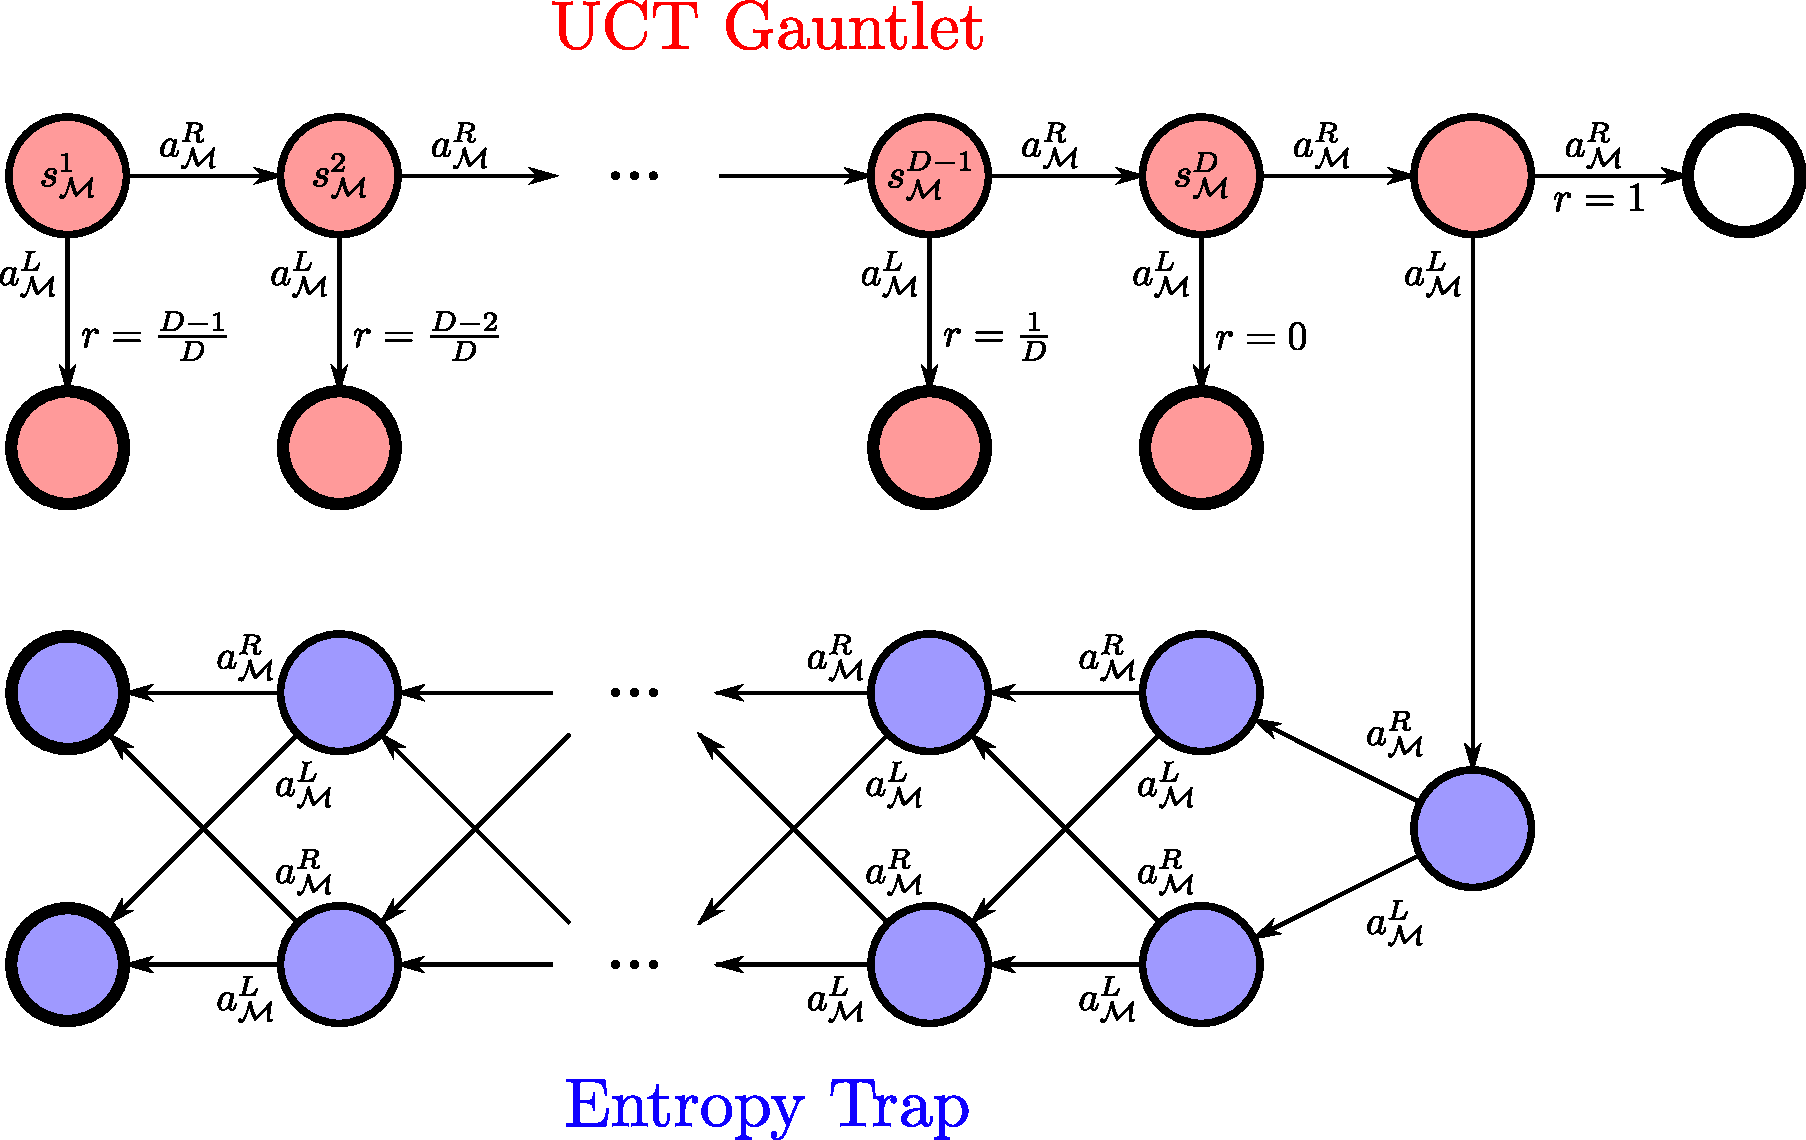
\includegraphics[width=\textwidth]{figures/ch4/entropy_trap_mdp_colour.pdf}
            \caption[An illustration of the \textit{Entropy Trap problem}.]{An illustration of the \textit{Entropy Trap problem}. In red, the original D-chain problem (Figure \ref{fig:modified_d_chain}) is labelled as the UCT Gauntlet, and the additional states added for the Entropy Trap are in blue. If a reward is not specified for a transition it is zero. \todo{this fig is copied, update caption?}}
            \label{fig:entropy_trap_repeat}
        \end{figure}
        
        
        
        \begin{theorem} \label{thrm:ments_bad_mdp}
            Consider a MENTS process with arbitrary temperature $\alphaments$. There exists and MDP such that for any $\alphaments$ that MENTS is either not consistent, or requires an exponential number of trials in the size of the state space. More precisely, either $\mathbb{E}\sreg(s_0,\mpsiments{n})\not\rightarrow 0$ or $\mathbb{E}\sreg(1,\mpsiments{n}) \geq c(1 - \frac{n}{k^{|\cl{S}|}})$, which implies that $\mathbb{E}\sreg(s_0,\psi^n_{MENTS})>0$ for $n<k^{|\cl{S}|}$. \todo{make sure this has same label and same notation as in Sec 4.3}
        \end{theorem}
        
        \begin{proofoutline}
            \todo{remember this one was written in a bit of a rush, so probably want to make it a little clearer. Also need to make it consistent with the states and actions notation} 

            \todo{Also a bunch of N(s) instead of N(s,n) in the proof that need to be fixed}

            Proof is by construction. Consider the adapted-chain MDP \todo{update name for name change?} defined in Figure \ref{fig:entropy_trap_repeat}, which is parameterised by $D$ the length of the UCT gauntlet, and $K$, half the number of states in the entropy trap. To prove the claim, two cases need to be considered: when the temperature is sufficiently high for MENTS to get `caught' in the entropy trap when it is inconsistent; and, when the temperature is lower than this threshold.
            
            Case 1: $\alphaments>\frac{1}{\log(2)K}$ (MENTS gets caught by the entropy trap).
            
            If $\alphaments>\frac{1}{\log(2)K}$, the soft value of E is greater than one for any policy over the actions, and $\phi$ is a uniform policy (note that because there are no MDP rewards after $E$, $\phi$ is both the initial policy for MENTS and the optimal soft policy \todo{only for the entropy trap section}): 
            \begin{align}
                    V_{\sft}^*(E) & = 0 + \alphaments \cdot \mathcal{H}(\phi) \\
                        & = \alphaments \cdot \log(2)  K \\
                        & > 1 \\
                        & = V_{\sft}^*(F).
            \end{align}
            
            Hence the optimal soft values (which MENTS converges to) will recommend going to state $E$ and gathering $0$ reward. Hence in this case the simple regret will converge to $1$ as the optimal value is $V^*(1)=1$. That is $\mathbb{E}\sreg(1,\mpsiments{n}) \rightarrow 1 > 0$.
            
            Case 2: $\alpha\leq\frac{1}{\log(2)K}$ \todo{asnother comment on this case, or remove comment from other case}
            
            In this case it is argued that with a low $\alphaments$ that MENTS will only have a low probability of ever hitting state $D$, that is, it requires a lot of trials to garuntee that at least one trial has reached state $D$, which is necessary to get the reward of $1$ (and simple regret of $0$).
            
            First consider the composed and simplified soft backup on the adapted-chain problem for any $0<i<D$ to get:
            \begin{align}
                    \mVments{N(i,n)}(i) & = \alpha \log\left( \frac{1}{\alpha} 
                        \left( \frac{D-i}{D} + \mVments{N(i+1,n)}(i+1) \right)\right) \\
                    & \leq \max\left(\frac{D-i}{D},\mVments{N(i+1,n)}(i+1)\right) + \alpha\log(2) \label{mbm:one} \\
                    & \leq \max\left(\frac{D-i}{D},\mVments{N(i+1,n)}(i+1)\right) + \frac{1}{K}
            \end{align}
            
            where inequality (\ref{mbm:one}) used the property of log-sum-exp that $\alpha \log \sum_{i=1}^\ell \exp (x_i/\alpha) \leq \max_i (x_i) + \alpha \log(\ell)$. Assume that $K \geq D$ and $\mVments{N(D)}(D)=0$ (it will be checked that these assumptions are valid later). Then, by induction, it holds that $\mVments{N(i)}(i)\leq \frac{D-(i-1)}{D}$:
            \begin{align}
                \mVments{N(i)}(i) 
                & \leq \max\left(\frac{D-i}{D},\mVments{N(i+1)}(i+1)\right) + \frac{\log(2)}{\log(K)} \\
                & \leq \frac{D-i}{D} + \frac{1}{K} \\
                & \leq \frac{D-i}{D} + \frac{1}{D} \\
                & = \frac{D-(i-1)}{D}.
            \end{align}
            %
            \todo{first line uses induction hypothesis, value at i plus one less than D-i/D.}
            
            Now let the event $Y(n)$ be that MENTS visits state $D$ in its $n$th trial. Again assuming that $\mVments{N(D,n)}(D)=0$, the probability of this event occuring is less than $2^{-D}$. Because given this assumption it has just been shown that $\mVments{N(i+1,n)}(i+1)\leq \frac{D-i}{D} = \mVments{N(G_{i},n)}(G_{i})$, \todo{we are considering the choice between Gi and i plus 1 from state i here, which isn't too clear right now} as there are only two actions and taking action $a_R$ to continue down the chain has a lower soft value estimate, it must be that $\mpiments{n}(a_R|i) < \frac{1}{2}$, and as such, it must be that $\Pr\left(Y(n) \middle| \mVments{N(D,n)}(D)=0\right) < \frac{1}{2^D}$. 
            
            Then let $Z(n)=\neg \bigcup_{j=1}^n Y(j)$ be the event that no trial of MENTS has visited state $D$ in any of the first $n$ trials. And note that $Z(n)$ implies that $\mVments{N(D,n)}(D)=0$: \todo{probably aught to say somewhere in the proofs section that all the initialisations are set to zero, and the theory is to analyse the algorithms by itself, without any informative prior knowledge of the mdp}
            \begin{align}
                \Pr(Z(n)) 
                    &= \Pr\left(Z(n) \cap \mVments{N(D,n)}(D)=0\right) \\
                    &= \Pr\left(\neg Y(n) \cap Z(n-1) \cap \mVments{N(D,n)}(D) = 0  \right) \\
                    &= \Pr\left(\neg Y(n) \middle| Z(n-1) \cap \mVments{N(D,n)}(D) = 0 \right) 
                        \Pr\left( Z(n-1) \cap \mVments{N(D,n)}(D) = 0 \right) \\
                    &\geq (1-2^{-D}) \Pr\left( Z(n-1) \cap \mVments{N(D,n)}(D) = 0 \right) \\
                    &= ... \\
                    &\geq (1-2^{-D})^n \Pr\left( Z(0) \cap \mVments{N(D)}(D)=0\right) \\
                    &= (1-2^{-D})^n \\
                    &\geq 1-n2^{-D},
            \end{align}
            where the penultimate line used $\Pr\left( Z(0) \cap \left(\mVments{N(D)}(D)=0\right)\right)=1$, as $Z(0)$ and $\mVments{N(D,n)}(D)=0$ are vacuously true at the start of running the algorithm, and in the final line used Bernoulli's inequality \todo{ref}.
            
            Informally, $Z(n)$ implies that $V^{\mpsiments{n}}(1) \leq \frac{9}{10}$, as no trial has even reached $D$ to be able to reach the reward of $1$ from $F$. And hence the expected simple regret in this environment of MENTS can be bounded below as follows:
            \begin{align}
                \mathbb{E}\sreg(1,\psi^n_{\text{MENTS}}) 
                    & \geq \left(1-\frac{9}{10}\right) \Pr(Z(n)) \\
                    & \geq \frac{1}{10} \left( 1-n2^{-D} \right).
            \end{align}
            
            Finally, setting $K=D$, so that $|\cl{S}|=4D+3<5D$ for $D\in\bb{N}$ \todo{D more than 1} and so $D=\frac{|\cl{S}|-3}{4}>\frac{|S|}{5}$. Substituting this into the above inequality gives $\mathbb{E}\sreg(1,\mpsiments{n}) \geq 1 - \frac{n}{\sqrt[5]{2}^{|S|}}$, which is greater than $0$ for $n < \sqrt[5]{2}^{|S|}$. That is $c=\frac{1}{10}$ and $k=\sqrt[5]{2}$.
        \end{proofoutline}


        \todo{Some note about how DENTS can handle this case by using entropy and then ignoring it for the recommendations. Moreover, by allowing the entropy temperature (beta) to be decayed, allows the entropy trap estimates to correctly converge to the correct value of zero, and could handle a case where there is something more complex than a single state with a reward of one when not taking the entropy trap.}

        \todo{Additionally, note that because the proofs for convergence for DENTS have constraints on parameters (or no constraints on params) that even on this case it will converge to the correct result.}










        



